% Options for packages loaded elsewhere
\PassOptionsToPackage{unicode}{hyperref}
\PassOptionsToPackage{hyphens}{url}
\PassOptionsToPackage{dvipsnames,svgnames,x11names}{xcolor}
%
\documentclass[
  letterpaper,
  DIV=11,
  numbers=noendperiod]{scrartcl}

\usepackage{amsmath,amssymb}
\usepackage{iftex}
\ifPDFTeX
  \usepackage[T1]{fontenc}
  \usepackage[utf8]{inputenc}
  \usepackage{textcomp} % provide euro and other symbols
\else % if luatex or xetex
  \usepackage{unicode-math}
  \defaultfontfeatures{Scale=MatchLowercase}
  \defaultfontfeatures[\rmfamily]{Ligatures=TeX,Scale=1}
\fi
\usepackage{lmodern}
\ifPDFTeX\else  
    % xetex/luatex font selection
\fi
% Use upquote if available, for straight quotes in verbatim environments
\IfFileExists{upquote.sty}{\usepackage{upquote}}{}
\IfFileExists{microtype.sty}{% use microtype if available
  \usepackage[]{microtype}
  \UseMicrotypeSet[protrusion]{basicmath} % disable protrusion for tt fonts
}{}
\makeatletter
\@ifundefined{KOMAClassName}{% if non-KOMA class
  \IfFileExists{parskip.sty}{%
    \usepackage{parskip}
  }{% else
    \setlength{\parindent}{0pt}
    \setlength{\parskip}{6pt plus 2pt minus 1pt}}
}{% if KOMA class
  \KOMAoptions{parskip=half}}
\makeatother
\usepackage{xcolor}
\setlength{\emergencystretch}{3em} % prevent overfull lines
\setcounter{secnumdepth}{5}
% Make \paragraph and \subparagraph free-standing
\ifx\paragraph\undefined\else
  \let\oldparagraph\paragraph
  \renewcommand{\paragraph}[1]{\oldparagraph{#1}\mbox{}}
\fi
\ifx\subparagraph\undefined\else
  \let\oldsubparagraph\subparagraph
  \renewcommand{\subparagraph}[1]{\oldsubparagraph{#1}\mbox{}}
\fi

\usepackage{color}
\usepackage{fancyvrb}
\newcommand{\VerbBar}{|}
\newcommand{\VERB}{\Verb[commandchars=\\\{\}]}
\DefineVerbatimEnvironment{Highlighting}{Verbatim}{commandchars=\\\{\}}
% Add ',fontsize=\small' for more characters per line
\usepackage{framed}
\definecolor{shadecolor}{RGB}{241,243,245}
\newenvironment{Shaded}{\begin{snugshade}}{\end{snugshade}}
\newcommand{\AlertTok}[1]{\textcolor[rgb]{0.68,0.00,0.00}{#1}}
\newcommand{\AnnotationTok}[1]{\textcolor[rgb]{0.37,0.37,0.37}{#1}}
\newcommand{\AttributeTok}[1]{\textcolor[rgb]{0.40,0.45,0.13}{#1}}
\newcommand{\BaseNTok}[1]{\textcolor[rgb]{0.68,0.00,0.00}{#1}}
\newcommand{\BuiltInTok}[1]{\textcolor[rgb]{0.00,0.23,0.31}{#1}}
\newcommand{\CharTok}[1]{\textcolor[rgb]{0.13,0.47,0.30}{#1}}
\newcommand{\CommentTok}[1]{\textcolor[rgb]{0.37,0.37,0.37}{#1}}
\newcommand{\CommentVarTok}[1]{\textcolor[rgb]{0.37,0.37,0.37}{\textit{#1}}}
\newcommand{\ConstantTok}[1]{\textcolor[rgb]{0.56,0.35,0.01}{#1}}
\newcommand{\ControlFlowTok}[1]{\textcolor[rgb]{0.00,0.23,0.31}{#1}}
\newcommand{\DataTypeTok}[1]{\textcolor[rgb]{0.68,0.00,0.00}{#1}}
\newcommand{\DecValTok}[1]{\textcolor[rgb]{0.68,0.00,0.00}{#1}}
\newcommand{\DocumentationTok}[1]{\textcolor[rgb]{0.37,0.37,0.37}{\textit{#1}}}
\newcommand{\ErrorTok}[1]{\textcolor[rgb]{0.68,0.00,0.00}{#1}}
\newcommand{\ExtensionTok}[1]{\textcolor[rgb]{0.00,0.23,0.31}{#1}}
\newcommand{\FloatTok}[1]{\textcolor[rgb]{0.68,0.00,0.00}{#1}}
\newcommand{\FunctionTok}[1]{\textcolor[rgb]{0.28,0.35,0.67}{#1}}
\newcommand{\ImportTok}[1]{\textcolor[rgb]{0.00,0.46,0.62}{#1}}
\newcommand{\InformationTok}[1]{\textcolor[rgb]{0.37,0.37,0.37}{#1}}
\newcommand{\KeywordTok}[1]{\textcolor[rgb]{0.00,0.23,0.31}{#1}}
\newcommand{\NormalTok}[1]{\textcolor[rgb]{0.00,0.23,0.31}{#1}}
\newcommand{\OperatorTok}[1]{\textcolor[rgb]{0.37,0.37,0.37}{#1}}
\newcommand{\OtherTok}[1]{\textcolor[rgb]{0.00,0.23,0.31}{#1}}
\newcommand{\PreprocessorTok}[1]{\textcolor[rgb]{0.68,0.00,0.00}{#1}}
\newcommand{\RegionMarkerTok}[1]{\textcolor[rgb]{0.00,0.23,0.31}{#1}}
\newcommand{\SpecialCharTok}[1]{\textcolor[rgb]{0.37,0.37,0.37}{#1}}
\newcommand{\SpecialStringTok}[1]{\textcolor[rgb]{0.13,0.47,0.30}{#1}}
\newcommand{\StringTok}[1]{\textcolor[rgb]{0.13,0.47,0.30}{#1}}
\newcommand{\VariableTok}[1]{\textcolor[rgb]{0.07,0.07,0.07}{#1}}
\newcommand{\VerbatimStringTok}[1]{\textcolor[rgb]{0.13,0.47,0.30}{#1}}
\newcommand{\WarningTok}[1]{\textcolor[rgb]{0.37,0.37,0.37}{\textit{#1}}}

\providecommand{\tightlist}{%
  \setlength{\itemsep}{0pt}\setlength{\parskip}{0pt}}\usepackage{longtable,booktabs,array}
\usepackage{calc} % for calculating minipage widths
% Correct order of tables after \paragraph or \subparagraph
\usepackage{etoolbox}
\makeatletter
\patchcmd\longtable{\par}{\if@noskipsec\mbox{}\fi\par}{}{}
\makeatother
% Allow footnotes in longtable head/foot
\IfFileExists{footnotehyper.sty}{\usepackage{footnotehyper}}{\usepackage{footnote}}
\makesavenoteenv{longtable}
\usepackage{graphicx}
\makeatletter
\def\maxwidth{\ifdim\Gin@nat@width>\linewidth\linewidth\else\Gin@nat@width\fi}
\def\maxheight{\ifdim\Gin@nat@height>\textheight\textheight\else\Gin@nat@height\fi}
\makeatother
% Scale images if necessary, so that they will not overflow the page
% margins by default, and it is still possible to overwrite the defaults
% using explicit options in \includegraphics[width, height, ...]{}
\setkeys{Gin}{width=\maxwidth,height=\maxheight,keepaspectratio}
% Set default figure placement to htbp
\makeatletter
\def\fps@figure{htbp}
\makeatother

\usepackage{booktabs}
\usepackage{longtable}
\usepackage{array}
\usepackage{multirow}
\usepackage{wrapfig}
\usepackage{float}
\usepackage{colortbl}
\usepackage{pdflscape}
\usepackage{tabu}
\usepackage{threeparttable}
\usepackage{threeparttablex}
\usepackage[normalem]{ulem}
\usepackage{makecell}
\usepackage{xcolor}
\KOMAoption{captions}{tableheading}
\usepackage{float}
\floatplacement{table}{H}
\floatplacement{figure}{H}
\makeatletter
\@ifpackageloaded{caption}{}{\usepackage{caption}}
\AtBeginDocument{%
\ifdefined\contentsname
  \renewcommand*\contentsname{Tabla de contenidos}
\else
  \newcommand\contentsname{Tabla de contenidos}
\fi
\ifdefined\listfigurename
  \renewcommand*\listfigurename{Listado de Figuras}
\else
  \newcommand\listfigurename{Listado de Figuras}
\fi
\ifdefined\listtablename
  \renewcommand*\listtablename{Listado de Tablas}
\else
  \newcommand\listtablename{Listado de Tablas}
\fi
\ifdefined\figurename
  \renewcommand*\figurename{Figura}
\else
  \newcommand\figurename{Figura}
\fi
\ifdefined\tablename
  \renewcommand*\tablename{Tabla}
\else
  \newcommand\tablename{Tabla}
\fi
}
\@ifpackageloaded{float}{}{\usepackage{float}}
\floatstyle{ruled}
\@ifundefined{c@chapter}{\newfloat{codelisting}{h}{lop}}{\newfloat{codelisting}{h}{lop}[chapter]}
\floatname{codelisting}{Listado}
\newcommand*\listoflistings{\listof{codelisting}{Listado de Listados}}
\makeatother
\makeatletter
\makeatother
\makeatletter
\@ifpackageloaded{caption}{}{\usepackage{caption}}
\@ifpackageloaded{subcaption}{}{\usepackage{subcaption}}
\makeatother
\ifLuaTeX
\usepackage[bidi=basic]{babel}
\else
\usepackage[bidi=default]{babel}
\fi
\babelprovide[main,import]{spanish}
% get rid of language-specific shorthands (see #6817):
\let\LanguageShortHands\languageshorthands
\def\languageshorthands#1{}
\ifLuaTeX
  \usepackage{selnolig}  % disable illegal ligatures
\fi
\usepackage{bookmark}

\IfFileExists{xurl.sty}{\usepackage{xurl}}{} % add URL line breaks if available
\urlstyle{same} % disable monospaced font for URLs
\hypersetup{
  pdftitle={Datos del Viaje},
  pdfauthor={María Varela Oyola},
  pdflang={es},
  colorlinks=true,
  linkcolor={blue},
  filecolor={Maroon},
  citecolor={Blue},
  urlcolor={Blue},
  pdfcreator={LaTeX via pandoc}}

\title{Datos del Viaje}
\author{María Varela Oyola}
\date{10/11/2025}

\begin{document}
\maketitle

\renewcommand*\contentsname{Tabla de contenidos}
{
\hypersetup{linkcolor=}
\setcounter{tocdepth}{4}
\tableofcontents
}
\pagebreak

\section{Planteamiento}\label{planteamiento}

El objetivo de este trabajo es seleccionar el mejor destino para
realizar un viaje en familia (compuesta por 5 personas) durante las
vacaciones de Navidad, aplicando distintas técnicas de decisión
multicriterio vistas en clase (AHP, ELECTRE, PROMETHEE).\\
Para ello se han definido cuatro alternativas que representan diferentes
tipos de experiencias navideñas en Europa, y se han establecido
criterios de evaluación que permiten comparar sus ventajas y
desventajas.

\subsection{Alternativas propuestas}\label{alternativas-propuestas}

Definiremos las cuatro ciudades europeas seleccionadas como posibles
destinos para realizar un viaje durante las vacaciones de Navidad. Cada
una ofrece un tipo de experiencia diferente (desde la tradición más
clásica hasta la combinación de cultura, historia y modernidad), lo que
las convierte en alternativas idóneas para aplicar técnicas de decisión
multicriterio.

\subsubsection{Colonia (Alemania)}\label{colonia-alemania}

Colonia es una de las ciudades más antiguas de Alemania, situada a
orillas del río Rin. Es reconocida por su Catedral gótica, una obra
maestra declarada Patrimonio de la Humanidad por la UNESCO, y por su
ambiente cosmopolita y acogedor. La ciudad combina una rica historia
romana y medieval con una intensa vida moderna, destacando por su arte
contemporáneo, su escena musical y sus festivales.

Entre sus principales atractivos se encuentran el Museo Ludwig (arte
moderno y pop), el Museo Romano-Germánico, el paseo por el Rin y sus
tradicionales cervecerías donde se sirve la cerveza Kölsch, típica de la
región.

Durante diciembre, Colonia se transforma en un destino navideño de
referencia en Europa. La ciudad acoge más de seis mercados navideños
repartidos por distintas plazas, siendo el más famoso el situado frente
a la Catedral.

\begin{figure}[H]

{\centering \includegraphics[width=2.34375in,height=\textheight]{Que-ver-en-Colonia.png}

}

\caption{Imagen panorámica de Colonia, Alemania}

\end{figure}%

\subsubsection{Florencia (Italia)}\label{florencia-italia}

Florencia, capital de la región de la Toscana, es una de las ciudades
más bellas e influyentes del mundo. Considerada la cuna del
Renacimiento, ha sido hogar de grandes artistas como Miguel Ángel,
Leonardo da Vinci o Brunelleschi. Pasear por sus calles es recorrer
siglos de arte e historia.

Sus principales atractivos incluyen la Catedral de Santa Maria del Fiore
con su cúpula icónica, el Ponte Vecchio, la Galería Uffizi y el Palazzo
Vecchio. Además, Florencia destaca por su gastronomía toscana, su vino
Chianti y sus trattorias tradicionales.

Durante la Navidad, la ciudad se ilumina con el F-Light Festival, un
espectáculo de proyecciones y luces sobre sus monumentos, y el mercado
navideño de la Piazza Santa Croce, inspirado en la tradición alemana.
Aunque las celebraciones son más discretas que en el norte de Europa, el
ambiente es elegante y acogedor, perfecto para quienes buscan una
Navidad cultural y gastronómica.

Florencia es, en cualquier época del año, un destino excepcional para
los amantes del arte, la historia y la buena cocina, ofreciendo una
experiencia refinada y profundamente italiana.

\begin{figure}[H]

{\centering 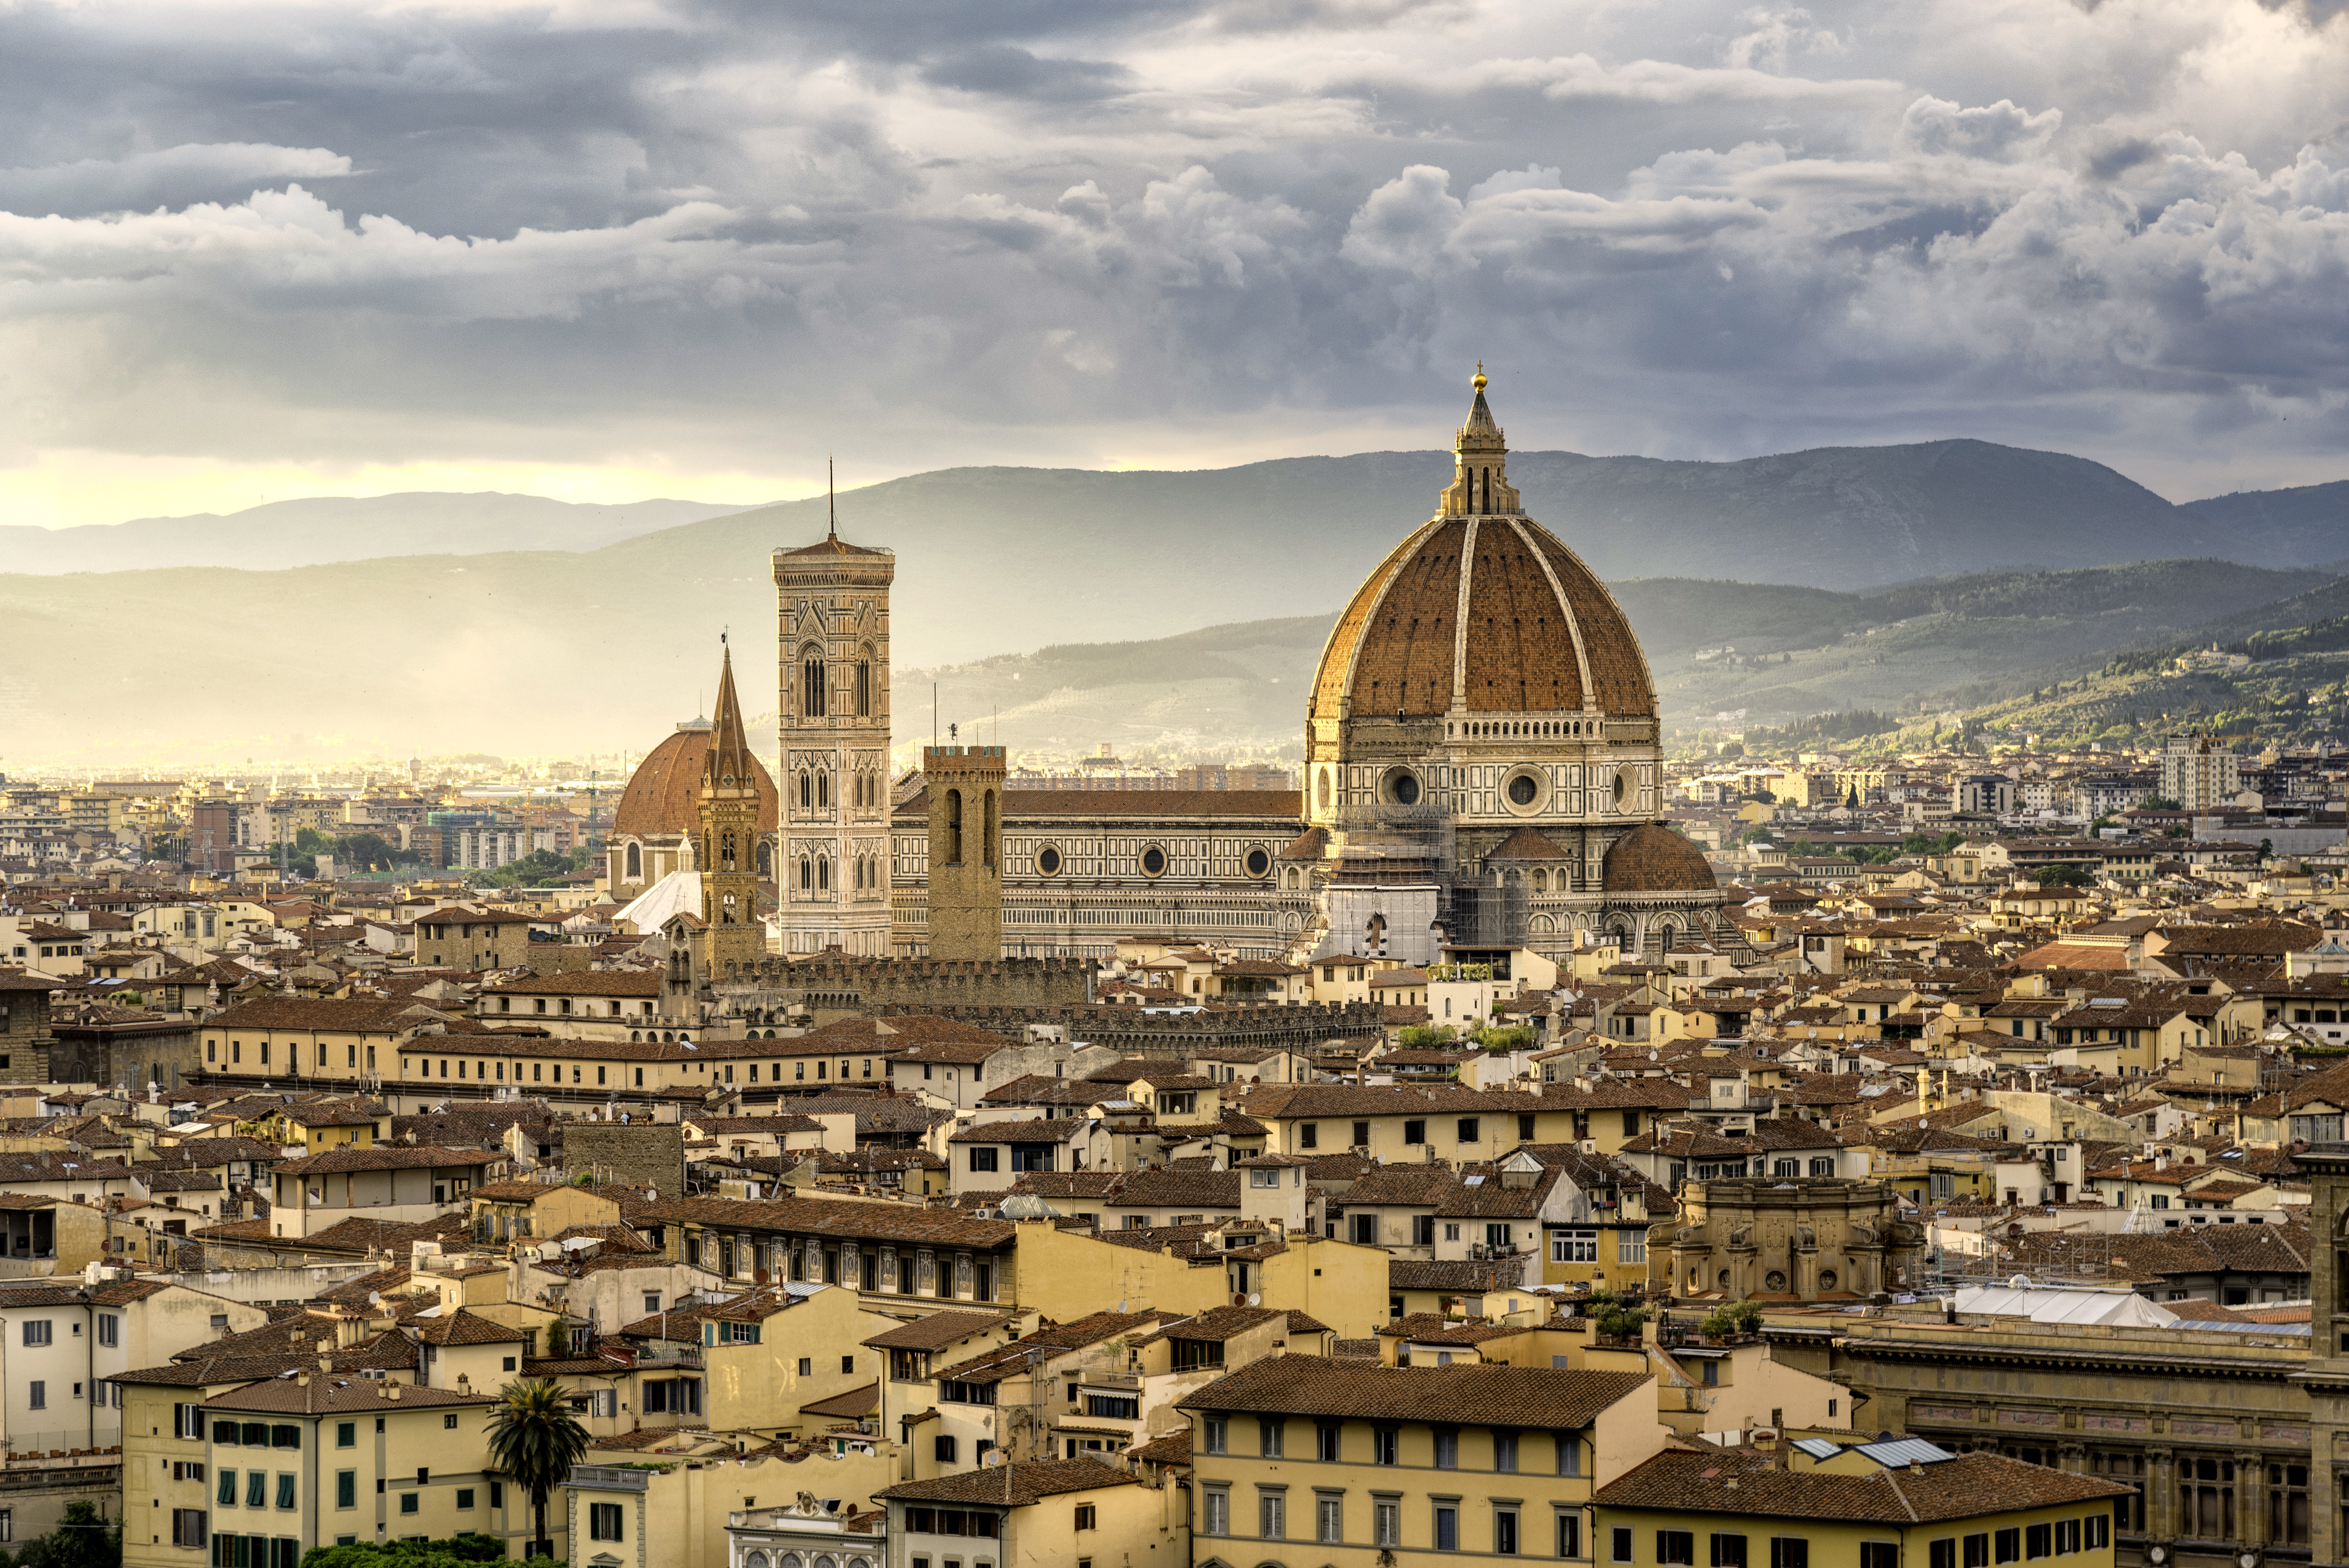
\includegraphics[width=2.34375in,height=\textheight]{foto1.png}

}

\caption{Imagen panorámica de Florencia, Italia}

\end{figure}%

\subsubsection{Estrasburgo (Francia)}\label{estrasburgo-francia}

Situada en la región de Alsacia, en la frontera entre Francia y
Alemania, Estrasburgo combina lo mejor de ambas culturas. Su casco
histórico, la Grande Île, está declarado Patrimonio Mundial por la
UNESCO por su arquitectura gótica y sus canales pintorescos. La ciudad
es también sede del Parlamento Europeo, lo que le da un carácter
internacional y dinámico.

Estrasburgo es una ciudad de escala humana, ideal para recorrer a pie o
en bicicleta. Su Catedral de Notre-Dame, una joya del gótico tardío,
domina el paisaje urbano. Los barrios de La Petite France y Krusenstern
ofrecen un encanto singular con casas de entramado de madera, puentes y
calles adoquinadas.

Durante diciembre, la ciudad se convierte en un auténtico símbolo de la
Navidad europea. El mercado Christkindelsmärik (el más antiguo del
continente, fundado en 1570) llena la ciudad de vida, luces y tradición.
La gastronomía alsaciana, con platos como el bäckeoffe o los bredele,
refleja la fusión franco-alemana.

\begin{figure}[H]

{\centering \includegraphics[width=2.42708in,height=\textheight]{foto2.png}

}

\caption{Imagen panorámica de Estrasburgo, Francia}

\end{figure}%

\subsubsection{Edimburgo (Escocia, Reino
Unido)}\label{edimburgo-escocia-reino-unido}

Edimburgo, es una ciudad de contrastes: combina una arquitectura
medieval impresionante con una vibrante vida cultural y artística. Su
perfil, dominado por el Castillo de Edimburgo sobre una colina
volcánica, es uno de los más reconocibles de Europa.

La ciudad ofrece dos zonas claramente diferenciadas: la Old Town, de
calles empedradas y ambiente histórico, y la New Town, planificada en el
siglo XVIII con elegantes avenidas georgianas. Entre sus principales
atractivos destacan el Royal Mile, el Palacio de Holyrood, el Arthur's
Seat (una colina con vistas panorámicas) y los numerosos museos y
festivales culturales.

Durante el invierno, Edimburgo adquiere una atmósfera mágica: el mercado
navideño de Princes Street Gardens ofrece artesanía, gastronomía y
atracciones; mientras que el Hogmanay, su famoso festival de Año Nuevo,
es uno de los más espectaculares del mundo, con desfiles, conciertos y
fuegos artificiales.

\begin{figure}[H]

{\centering \includegraphics[width=2.34375in,height=\textheight]{foto4.png}

}

\caption{Imagen panorámica de Edimburgo, Escocia}

\end{figure}%

\pagebreak

\subsection{Criterios y subcriterios}\label{criterios-y-subcriterios}

\subsubsection{Vuelos}\label{vuelos}

El vuelo condiciona gran parte de la logística y la comodidad del viaje.
Es por ello que será uno de los criterios más importantes a la hora de
plantear este viaje. Los subcriterios a estudiar son:

\begin{itemize}
\item
  Hora de llegada:

  \begin{itemize}
  \item
    Explicación: Es preferible llegar cuanto antes para aprovechar el
    primer día.
  \item
    Preferencia: Cuanto menor sea el valor (es decir, más temprana sea
    la hora) mejor.
  \end{itemize}
\item
  Hora de vuelta:

  \begin{itemize}
  \item
    Explicación: Es preferible vuelos de regreso tardíos para aprovechar
    el día de salida.
  \item
    Preferencia: Cuanto mayor sea el valor (es decir, más tarde sea la
    hora) mejor.
  \end{itemize}
\item
  Precio del vuelo:

  \begin{itemize}
  \item
    Explicación: Al ser 5 viajeros, el precio es clave en el viaje,
    siendo el de los vuelos de los más relevantes.
  \item
    Preferencia: A menor valor, mejor.
  \end{itemize}
\end{itemize}

\subsubsection{Alojamiento}\label{alojamiento}

El alojamiento es un punto clave en este estudio, ya que al plantear el
estudio ante una familia de 5 personas, una sola habitación de hotel no
es viable, lo que obligaría a reservar dos habitaciones, encareciendo
considerablemente el viaje.

\begin{itemize}
\item
  Precio del alojamiento:

  \begin{itemize}
  \item
    Explicación: Buscamos alojamientos económicos, siendo clave para el
    precio del viaje.
  \item
    Preferencia: A menor valor, mejor.
  \end{itemize}
\item
  Tipo de alojamiento:

  \begin{itemize}
  \item
    Explicación: Debido a preferencias personales, se prefiere optar por
    un hotel en vez de un apartamento, es por ello que se tendrá en
    cuenta.
  \item
    Preferencia: Mejor un hotel
  \end{itemize}
\item
  Ubicación (centralidad):

  \begin{itemize}
  \item
    Explicación: Una ubicación céntrica reduce tiempo y coste en
    desplazamientos y facilita disfrutar del destino.
  \item
    Preferencia: A mayor centralidad mejor.
  \end{itemize}
\item
  Puntuación (valoraciones):

  \begin{itemize}
  \item
    Explicación: La puntuación refleja calidad, limpieza y servicio, lo
    que mejoraría el viaje.
  \item
    Preferencia: A mayor puntuación mejor.
  \end{itemize}
\end{itemize}

\subsubsection{Fecha}\label{fecha}

Las fechas influyen en disponibilidad, precios y compatibilidad con los
exámenes de enero, teniendo dos dimensiones temporales importantes.

\begin{itemize}
\item
  Días de viaje:

  \begin{itemize}
  \item
    Explicación: Cuantas más horas estemos en el destino, más
    aprovechamos el viaje y más cosas podemos ver.
  \item
    Preferencia: A mayor tiempo, mejor
  \end{itemize}
\item
  Días del mes:

  \begin{itemize}
  \item
    Explicación: Debido a los exámenes de enero, cuanto más alejada sea
    la fecha del viaje con respecto al 7 de enero, mejor
  \item
    Preferencia: A mayor distancia mejor.
  \end{itemize}
\end{itemize}

\subsubsection{Tiempo (clima)}\label{tiempo-clima}

El clima condiciona las actividades al aire libre y la estética del
viaje (nieve, frío, sol).

\begin{itemize}
\item
  Temperatura media:

  \begin{itemize}
  \item
    Explicación: Se prefieren temperaturas más suaves.
  \item
    Preferencia: A mayor temperatura mejor.
  \end{itemize}
\end{itemize}

\subsubsection{Comida}\label{comida}

La calidad y accesibilidad alimentaria influyen fuertemente en la
experiencia del viaje, especialmente teniendo en cuenta que un miembro
de la familia es celiaco.

\begin{itemize}
\item
  Accesibilidad a comidas sin gluten:

  \begin{itemize}
  \item
    Explicación: Disponibilidad de opciones sin gluten en restaurantes y
    supermercados.
  \item
    Preferencia: A mayor cobertura mejor.
  \end{itemize}
\item
  Precio medio de la comida:

  \begin{itemize}
  \item
    Explicación: El precio de la comida tiene un gran impacto en
    presupuesto, aumentando el coste total del viaje.
  \item
    Preferencia: A menor precio mejor.
  \end{itemize}
\end{itemize}

\subsubsection{Experiencia navideña}\label{experiencia-navideuxf1a}

Dado que nos vamos en fechas navideñas, es de tener en cuenta los
mercados navideños y la experiencia navideña que puede ofrecernos el
sitio del destino.

\begin{itemize}
\item
  Calidad de mercados navideños:

  \begin{itemize}
  \item
    Explicación: Se tiene en cuenta tamaño, variedad de puestos,
    tradición, ambientación y eventos asociados.
  \item
    Preferencia: A mayor puntuación mejor.
  \end{itemize}
\end{itemize}

\pagebreak

\section{Datos a utilizar en el
estudio}\label{datos-a-utilizar-en-el-estudio}

\subsection{Opciones de vuelos}\label{opciones-de-vuelos}

\textbf{Vuelos a Colonia}

\begin{longtable}[]{@{}
  >{\raggedright\arraybackslash}p{(\columnwidth - 10\tabcolsep) * \real{0.1667}}
  >{\raggedright\arraybackslash}p{(\columnwidth - 10\tabcolsep) * \real{0.1667}}
  >{\raggedright\arraybackslash}p{(\columnwidth - 10\tabcolsep) * \real{0.1667}}
  >{\raggedright\arraybackslash}p{(\columnwidth - 10\tabcolsep) * \real{0.1667}}
  >{\raggedright\arraybackslash}p{(\columnwidth - 10\tabcolsep) * \real{0.1667}}
  >{\raggedright\arraybackslash}p{(\columnwidth - 10\tabcolsep) * \real{0.1667}}@{}}
\caption{Vuelos Sevilla - Colonia}\tabularnewline
\toprule\noalign{}
\begin{minipage}[b]{\linewidth}\raggedright
Fecha
\end{minipage} & \begin{minipage}[b]{\linewidth}\raggedright
Aeropuerto salida
\end{minipage} & \begin{minipage}[b]{\linewidth}\raggedright
Hora salida
\end{minipage} & \begin{minipage}[b]{\linewidth}\raggedright
Aeropuerto llegada
\end{minipage} & \begin{minipage}[b]{\linewidth}\raggedright
Hora llegada
\end{minipage} & \begin{minipage}[b]{\linewidth}\raggedright
Precio
\end{minipage} \\
\midrule\noalign{}
\endfirsthead
\toprule\noalign{}
\begin{minipage}[b]{\linewidth}\raggedright
Fecha
\end{minipage} & \begin{minipage}[b]{\linewidth}\raggedright
Aeropuerto salida
\end{minipage} & \begin{minipage}[b]{\linewidth}\raggedright
Hora salida
\end{minipage} & \begin{minipage}[b]{\linewidth}\raggedright
Aeropuerto llegada
\end{minipage} & \begin{minipage}[b]{\linewidth}\raggedright
Hora llegada
\end{minipage} & \begin{minipage}[b]{\linewidth}\raggedright
Precio
\end{minipage} \\
\midrule\noalign{}
\endhead
\bottomrule\noalign{}
\endlastfoot
jueves 1 enero & SVQ Sevilla & 6:30 & CGN Colonia & 9:25 & 25€ \\
lunes 5 enero & CNG Colonia & 15:35 & SVQ Sevilla & 18:30 & 64€ \\
\end{longtable}

Dados los vuelos de ida y vuelta a Colonia desde Sevilla, vamos a
definir los datos que utilizaremos de cara a los subcriterios:

\begin{itemize}
\item
  La hora de llegada es: 9:25
\item
  La hora de vuelta es: 15:35
\item
  El precio del vuelo en total es de: 89€
\end{itemize}

\textbf{Vuelos a Florencia}

\begin{longtable}[]{@{}
  >{\raggedright\arraybackslash}p{(\columnwidth - 10\tabcolsep) * \real{0.1667}}
  >{\raggedright\arraybackslash}p{(\columnwidth - 10\tabcolsep) * \real{0.1667}}
  >{\raggedright\arraybackslash}p{(\columnwidth - 10\tabcolsep) * \real{0.1667}}
  >{\raggedright\arraybackslash}p{(\columnwidth - 10\tabcolsep) * \real{0.1667}}
  >{\raggedright\arraybackslash}p{(\columnwidth - 10\tabcolsep) * \real{0.1667}}
  >{\raggedright\arraybackslash}p{(\columnwidth - 10\tabcolsep) * \real{0.1667}}@{}}
\caption{Vuelos Sevilla - Pisa}\tabularnewline
\toprule\noalign{}
\begin{minipage}[b]{\linewidth}\raggedright
Fecha
\end{minipage} & \begin{minipage}[b]{\linewidth}\raggedright
Aeropuerto salida
\end{minipage} & \begin{minipage}[b]{\linewidth}\raggedright
Hora salida
\end{minipage} & \begin{minipage}[b]{\linewidth}\raggedright
Aeropuerto llegada
\end{minipage} & \begin{minipage}[b]{\linewidth}\raggedright
Hora llegada
\end{minipage} & \begin{minipage}[b]{\linewidth}\raggedright
Precio
\end{minipage} \\
\midrule\noalign{}
\endfirsthead
\toprule\noalign{}
\begin{minipage}[b]{\linewidth}\raggedright
Fecha
\end{minipage} & \begin{minipage}[b]{\linewidth}\raggedright
Aeropuerto salida
\end{minipage} & \begin{minipage}[b]{\linewidth}\raggedright
Hora salida
\end{minipage} & \begin{minipage}[b]{\linewidth}\raggedright
Aeropuerto llegada
\end{minipage} & \begin{minipage}[b]{\linewidth}\raggedright
Hora llegada
\end{minipage} & \begin{minipage}[b]{\linewidth}\raggedright
Precio
\end{minipage} \\
\midrule\noalign{}
\endhead
\bottomrule\noalign{}
\endlastfoot
miércoles 31 diciembre & SVQ Sevilla & 10:30 & PSA Pisa & 13:05 & 28€ \\
domingo 4 enero & PSA Pisa & 8:00 & SVQ Sevilla & 10:35 & 65€ \\
\end{longtable}

Dados los vuelos de ida y vuelta a Florencia (con conexión al aeropuerto
de Pisa) desde Sevilla, vamos a definir los datos que utilizaremos de
cara a los subcriterios:

\begin{itemize}
\item
  La hora de llegada es: 13:05
\item
  La hora de vuelta es: 8:00
\item
  El precio del vuelo en total es de: 93€
\end{itemize}

\textbf{Vuelos a Estrasburgo}

\begin{longtable}[]{@{}
  >{\raggedright\arraybackslash}p{(\columnwidth - 10\tabcolsep) * \real{0.1667}}
  >{\raggedright\arraybackslash}p{(\columnwidth - 10\tabcolsep) * \real{0.1667}}
  >{\raggedright\arraybackslash}p{(\columnwidth - 10\tabcolsep) * \real{0.1667}}
  >{\raggedright\arraybackslash}p{(\columnwidth - 10\tabcolsep) * \real{0.1667}}
  >{\raggedright\arraybackslash}p{(\columnwidth - 10\tabcolsep) * \real{0.1667}}
  >{\raggedright\arraybackslash}p{(\columnwidth - 10\tabcolsep) * \real{0.1667}}@{}}
\caption{Vuelos Sevilla - Baden Baden}\tabularnewline
\toprule\noalign{}
\begin{minipage}[b]{\linewidth}\raggedright
Fecha
\end{minipage} & \begin{minipage}[b]{\linewidth}\raggedright
Aeropuerto salida
\end{minipage} & \begin{minipage}[b]{\linewidth}\raggedright
Hora salida
\end{minipage} & \begin{minipage}[b]{\linewidth}\raggedright
Aeropuerto llegada
\end{minipage} & \begin{minipage}[b]{\linewidth}\raggedright
Hora llegada
\end{minipage} & \begin{minipage}[b]{\linewidth}\raggedright
Precio
\end{minipage} \\
\midrule\noalign{}
\endfirsthead
\toprule\noalign{}
\begin{minipage}[b]{\linewidth}\raggedright
Fecha
\end{minipage} & \begin{minipage}[b]{\linewidth}\raggedright
Aeropuerto salida
\end{minipage} & \begin{minipage}[b]{\linewidth}\raggedright
Hora salida
\end{minipage} & \begin{minipage}[b]{\linewidth}\raggedright
Aeropuerto llegada
\end{minipage} & \begin{minipage}[b]{\linewidth}\raggedright
Hora llegada
\end{minipage} & \begin{minipage}[b]{\linewidth}\raggedright
Precio
\end{minipage} \\
\midrule\noalign{}
\endhead
\bottomrule\noalign{}
\endlastfoot
miércoles 31 diciembre & SVQ Sevilla & 17:25 & FKB Karlsruhe /
Baden-Baden & 20:05 & 45€ \\
lunes 5 enero & FKB Karlsruhe / Baden-Baden & 15:10 & SVQ Sevilla &
17:50 & 55€ \\
\end{longtable}

Dados los vuelos de ida y vuelta a Estrasburgo (con conexión al
aeropuerto de Karlsruhe / Baden-Baden) desde Sevilla, vamos a definir
los datos que utilizaremos de cara a los subcriterios:

\begin{itemize}
\item
  La hora de llegada es: 20:05
\item
  La hora de vuelta es: 15:10
\item
  El precio del vuelo en total es de: 100€
\end{itemize}

\textbf{Vuelos a Edimburgo}

\begin{longtable}[]{@{}
  >{\raggedright\arraybackslash}p{(\columnwidth - 10\tabcolsep) * \real{0.1667}}
  >{\raggedright\arraybackslash}p{(\columnwidth - 10\tabcolsep) * \real{0.1667}}
  >{\raggedright\arraybackslash}p{(\columnwidth - 10\tabcolsep) * \real{0.1667}}
  >{\raggedright\arraybackslash}p{(\columnwidth - 10\tabcolsep) * \real{0.1667}}
  >{\raggedright\arraybackslash}p{(\columnwidth - 10\tabcolsep) * \real{0.1667}}
  >{\raggedright\arraybackslash}p{(\columnwidth - 10\tabcolsep) * \real{0.1667}}@{}}
\caption{Vuelos Sevilla - Edimburgo}\tabularnewline
\toprule\noalign{}
\begin{minipage}[b]{\linewidth}\raggedright
Fecha
\end{minipage} & \begin{minipage}[b]{\linewidth}\raggedright
Aeropuerto salida
\end{minipage} & \begin{minipage}[b]{\linewidth}\raggedright
Hora salida
\end{minipage} & \begin{minipage}[b]{\linewidth}\raggedright
Aeropuerto llegada
\end{minipage} & \begin{minipage}[b]{\linewidth}\raggedright
Hora llegada
\end{minipage} & \begin{minipage}[b]{\linewidth}\raggedright
Precio
\end{minipage} \\
\midrule\noalign{}
\endfirsthead
\toprule\noalign{}
\begin{minipage}[b]{\linewidth}\raggedright
Fecha
\end{minipage} & \begin{minipage}[b]{\linewidth}\raggedright
Aeropuerto salida
\end{minipage} & \begin{minipage}[b]{\linewidth}\raggedright
Hora salida
\end{minipage} & \begin{minipage}[b]{\linewidth}\raggedright
Aeropuerto llegada
\end{minipage} & \begin{minipage}[b]{\linewidth}\raggedright
Hora llegada
\end{minipage} & \begin{minipage}[b]{\linewidth}\raggedright
Precio
\end{minipage} \\
\midrule\noalign{}
\endhead
\bottomrule\noalign{}
\endlastfoot
martes 30 diciembre & SVQ Sevilla & 10:30 & EDI Edimburgo & 12:40 &
45€ \\
viernes 2 enero & EDI Edimburgo & 5:50 & SVQ Sevilla & 10:00 & 93€ \\
\end{longtable}

Dados los vuelos de ida y vuelta a Edimburgo desde Sevilla, vamos a
definir los datos que utilizaremos de cara a los subcriterios:

\begin{itemize}
\item
  La hora de llegada es: 12:40
\item
  La hora de vuelta es: 5:50
\item
  El precio del vuelo en total es de: 138€
\end{itemize}

\subsection{Opciones de alojamiento}\label{opciones-de-alojamiento}

\textbf{Alojamiento en Colonia}

\begin{longtable}[]{@{}llll@{}}
\caption{Alojamiento en Colonia}\tabularnewline
\toprule\noalign{}
Tipo (hotel/apart) & Puntuación & Ubicación & Precio \\
\midrule\noalign{}
\endfirsthead
\toprule\noalign{}
Tipo (hotel/apart) & Puntuación & Ubicación & Precio \\
\midrule\noalign{}
\endhead
\bottomrule\noalign{}
\endlastfoot
Hotel & 8 & 3,5 & 671€ \\
\end{longtable}

Dado el alojamiento de Colonia, vamos a definir los datos que
utilizaremos de cara a los subcriterios:

\begin{itemize}
\item
  El precio del alojamiento es: 671€
\item
  El alojamiento es: hotel
\item
  La ubicación es de: 3.5 km
\item
  La puntuación es de: 8
\end{itemize}

\textbf{Alojamiento en Florencia}

\begin{longtable}[]{@{}llll@{}}
\caption{Alojamiento en Florencia}\tabularnewline
\toprule\noalign{}
Tipo (hotel/apart) & Puntuación & Ubicación & Precio \\
\midrule\noalign{}
\endfirsthead
\toprule\noalign{}
Tipo (hotel/apart) & Puntuación & Ubicación & Precio \\
\midrule\noalign{}
\endhead
\bottomrule\noalign{}
\endlastfoot
Apartamento & 8,7 & 3,3 & 862€ \\
\end{longtable}

Dado el alojamiento de Florencia, vamos a definir los datos que
utilizaremos de cara a los subcriterios:

\begin{itemize}
\item
  El precio del alojamiento es: 862€
\item
  El alojamiento es: apartamento
\item
  La ubicación es de: 3.3 km
\item
  La puntuación es de: 8.7
\end{itemize}

\textbf{Alojamiento en Estrasburgo}

\begin{longtable}[]{@{}llll@{}}
\caption{Alojamiento en Estrasburgo}\tabularnewline
\toprule\noalign{}
Tipo (hotel/apart) & Puntuación & Ubicación & Precio \\
\midrule\noalign{}
\endfirsthead
\toprule\noalign{}
Tipo (hotel/apart) & Puntuación & Ubicación & Precio \\
\midrule\noalign{}
\endhead
\bottomrule\noalign{}
\endlastfoot
Apartamento & 9,4 & 0,9 & 1318€ \\
\end{longtable}

Dado el alojamiento de Estrasburgo, vamos a definir los datos que
utilizaremos de cara a los subcriterios:

\begin{itemize}
\item
  El precio del alojamiento es: 1318€
\item
  El alojamiento es: apartamento
\item
  La ubicación es de: 0.9 km
\item
  La puntuación es de: 9.4
\end{itemize}

\textbf{Alojamiento en Edimburgo}

\begin{longtable}[]{@{}llll@{}}
\caption{Alojamiento en Edimburgo}\tabularnewline
\toprule\noalign{}
Tipo (hotel/apart) & Puntuación & Ubicación & Precio \\
\midrule\noalign{}
\endfirsthead
\toprule\noalign{}
Tipo (hotel/apart) & Puntuación & Ubicación & Precio \\
\midrule\noalign{}
\endhead
\bottomrule\noalign{}
\endlastfoot
Apartamento & 7 & 4,8 & 1431€ \\
\end{longtable}

Dado el alojamiento de Edimburgo, vamos a definir los datos que
utilizaremos de cara a los subcriterios:

\begin{itemize}
\item
  El precio del alojamiento es: 1431€
\item
  El alojamiento es: apartamento
\item
  La ubicación es de: 4.8 km
\item
  La puntuación es de: 7
\end{itemize}

\subsection{Opciones de fechas}\label{opciones-de-fechas}

\textbf{Fechas de Colonia}

Definimos tanto las horas que estamos en el destino, como los días que
quedarían hasta el final de las vacaciones:

\begin{itemize}
\item
  Las horas que estamos en el destino son: 102 h
\item
  Los días que quedan hasta el 7 de enero son: 2
\end{itemize}

\textbf{Fechas de Florencia}

Definimos tanto las horas que estamos en el destino, como los días que
quedarían hasta el final de las vacaciones:

\begin{itemize}
\item
  Las horas que estamos en el destino son: 91 h
\item
  Los días que quedan hasta el 7 de enero son: 3
\end{itemize}

\textbf{Fechas de Estrasburgo}

Definimos tanto las horas que estamos en el destino, como los días que
quedarían hasta el final de las vacaciones:

\begin{itemize}
\item
  Las horas que estamos en el destino son: 115 h
\item
  Los días que quedan hasta el 7 de enero son: 2
\end{itemize}

\textbf{Fechas de Edimburgo}

Definimos tanto las horas que estamos en el destino, como los días que
quedarían hasta el final de las vacaciones:

\begin{itemize}
\item
  Las horas que estamos en el destino son: 65 h
\item
  Los días que quedan hasta el 7 de enero son: 5
\end{itemize}

\subsection{Opciones de Tiempo (clima)}\label{opciones-de-tiempo-clima}

\textbf{Clima de Colonia}

La temperatura media es de: 4º centígrados

\textbf{Clima de Florencia}

La temperatura media es de: 8º centígrados

\textbf{Clima de Estrasburgo}

La temperatura media es de: 2º centígrados

\textbf{Clima de Edimburgo}

La temperatura media es de: 3º centígrados

\subsection{Opciones de comida}\label{opciones-de-comida}

\textbf{Comida de Colonia}

\begin{itemize}
\item
  Número de restaurantes con opciones sin gluten: 8
\item
  Precio medio de la comida: 38€
\end{itemize}

\textbf{Comida de Florencia}

\begin{itemize}
\item
  Número de restaurantes con opciones sin gluten: 12
\item
  Precio medio de la comida: 40€
\end{itemize}

\textbf{Comida de Estrasburgo}

\begin{itemize}
\item
  Número de restaurantes con opciones sin gluten: 1
\item
  Precio medio de la comida: 32.5€
\end{itemize}

\textbf{Comida de Edimburgo}

\begin{itemize}
\item
  Número de restaurantes con opciones sin gluten: 9
\item
  Precio medio de la comida: 45.5€
\end{itemize}

\subsection{Opciones de experiencia
navideña}\label{opciones-de-experiencia-navideuxf1a}

\textbf{Experiencia navideña en Colonia}

La experiencia es de una puntuación de: 9

\textbf{Experiencia navideña en Florencia}

La experiencia es de una puntuación de: 7

\textbf{Experiencia navideña en Estrasburgo}

La experiencia es de una puntuación de: 10

\textbf{Experiencia navideña en Edimburgo}

La experiencia es de una puntuación de: 8

\pagebreak

\section{Cálculo de los pesos}\label{cuxe1lculo-de-los-pesos}

\subsection{Comparación de los criterios del
estudio}\label{comparaciuxf3n-de-los-criterios-del-estudio}

Vemos primero la comparación de los criterios principales, para
posteriormente ver la comparación de los subcriterios dentro de cada
criterio.

\begin{itemize}
\item
  Vuelos (mayor peso): se prioriza mucho la comodidad y coste del
  desplazamiento, ya que el viaje implica varios adultos y el
  presupuesto aéreo marca gran diferencia.
\item
  Alojamiento: también se considera muy relevante (solo ligeramente
  menos que vuelos), ya que el confort o el precio del alojamiento
  influye fuertemente en la satisfacción general.
\item
  Comida y Navidad: son de rango medio, debido a que se valoran como
  aspectos de disfrute más que de decisión práctica.
\item
  Fecha y tiempo (clima): se valoran mucho menos, luego se les da poca
  importancia relativa frente a los factores económicos o logísticos.
\end{itemize}

\begin{longtable}[]{@{}
  >{\raggedright\arraybackslash}p{(\columnwidth - 12\tabcolsep) * \real{0.1970}}
  >{\raggedright\arraybackslash}p{(\columnwidth - 12\tabcolsep) * \real{0.1212}}
  >{\raggedright\arraybackslash}p{(\columnwidth - 12\tabcolsep) * \real{0.1970}}
  >{\raggedright\arraybackslash}p{(\columnwidth - 12\tabcolsep) * \real{0.1061}}
  >{\raggedright\arraybackslash}p{(\columnwidth - 12\tabcolsep) * \real{0.1212}}
  >{\raggedright\arraybackslash}p{(\columnwidth - 12\tabcolsep) * \real{0.1212}}
  >{\raggedright\arraybackslash}p{(\columnwidth - 12\tabcolsep) * \real{0.1364}}@{}}
\caption{Comparación de criterios}\tabularnewline
\toprule\noalign{}
\endfirsthead
\endhead
\bottomrule\noalign{}
\endlastfoot
& Vuelos & Alojamiento & Fecha & Tiempo & Comida & Navidad \\
Vuelos & 1 & 2 & 7 & 9 & 8 & 7 \\
Alojamiento & 1/2 & 1 & 7 & 9 & 7 & 6 \\
Fecha & 1/7 & 1/7 & 1 & 1/3 & 1/4 & 3 \\
Tiempo & 1/9 & 1/9 & 3 & 1 & 1/5 & 1/2 \\
Comida & 1/8 & 1/7 & 4 & 5 & 1 & 6 \\
Navidad & 1/7 & 1/6 & 1/3 & 2 & 1/6 & 1 \\
\end{longtable}

\textbf{Comparación de los subcriterios del criterio vuelos:}

\begin{itemize}
\item
  Precio: domina completamente, ya que se busca minimizar costes.
\item
  Hora vuelta: es más importante que la hora de llegada, ya que afecta
  al aprovechamiento del último día del viaje (volver tarde permite más
  disfrute).
\end{itemize}

\begin{longtable}[]{@{}llll@{}}
\caption{Criterio: vuelos}\tabularnewline
\toprule\noalign{}
\endfirsthead
\endhead
\bottomrule\noalign{}
\endlastfoot
& Hora llegada & Hora vuelta & Precio \\
Hora llegada & 1 & 1/3 & 1/9 \\
Hora vuelta & 3 & 1 & 1/9 \\
Precio & 9 & 9 & 1 \\
\end{longtable}

\pagebreak

\textbf{Comparación de los subcriterios del criterio alojamiento:}

\begin{itemize}
\item
  Se prioriza el precio, seguido por la ubicación y la puntuación,
  porque el presupuesto es el factor dominante.
\item
  Tipo de alojamiento (hotel/apartamento): se considera poco relevante,
  pero hay una pequeña diferencia a la hora de preferir hotel
\end{itemize}

\begin{longtable}[]{@{}lllll@{}}
\caption{Criterio: alojamiento}\tabularnewline
\toprule\noalign{}
\endfirsthead
\endhead
\bottomrule\noalign{}
\endlastfoot
& Precio & Tipo & Ubicación & Puntuación \\
Precio & 1 & 8 & 7 & 6 \\
Tipo & 1/8 & 1 & 1/8 & 1/3 \\
Ubicación & 1/7 & 1/8 & 1 & 7 \\
Puntuación & 1/6 & 3 & 1/7 & 1 \\
\end{longtable}

\textbf{Comparación de los subcriterios del criterio fecha:}

\begin{itemize}
\tightlist
\item
  Se considera mucho más importante el número de horas aprovechables que
  el día concreto del mes, porque se busca maximizar el tiempo efectivo
  de viaje.
\end{itemize}

\begin{longtable}[]{@{}lll@{}}
\caption{Criterio: fecha}\tabularnewline
\toprule\noalign{}
\endfirsthead
\endhead
\bottomrule\noalign{}
\endlastfoot
& Horas & Día del mes \\
Horas & 1 & 8 \\
Día del mes & 1/8 & 1 \\
\end{longtable}

\textbf{Comparación de los subcriterios del criterio comida:}

\begin{itemize}
\item
  La disponibilidad de opciones sin gluten tiene un peso dominante,
  porque un viajero es celiaco y es prioritario que pueda tener opciones
  de comida durante el viaje.
\item
  El precio es relevante, pero claramente secundario.
\end{itemize}

\begin{longtable}[]{@{}lll@{}}
\caption{Criterio: comida}\tabularnewline
\toprule\noalign{}
\endfirsthead
\endhead
\bottomrule\noalign{}
\endlastfoot
& Sin gluten & Precio \\
Sin gluten & 1 & 5 \\
Precio & 1/5 & 1 \\
\end{longtable}

\subsection{Comparación de las
alternativas}\label{comparaciuxf3n-de-las-alternativas}

Realizamos una comparación de cada criterio y subcriterio según las
cuatro alternativas bajo estudio.

\textbf{Alternativas con respecto al criterio vuelos:}

\begin{itemize}
\item
  Hora llegada: más temprana es mejor, luego invertimos la escala (min =
  mejor).
\item
  Normalizamos con ratios aproximados:

  \begin{itemize}
  \item
    Colonia: 9:25 = 565 min
  \item
    Florencia: 13:05 = 785 mim
  \item
    Estrasburgo: 20:05 = 1205 min
  \item
    Edimburgo: 12:40 = 760 min
  \end{itemize}
\item
  min = mejor

  \begin{itemize}
  \item
    Colonia = 1205/565 = 2.13
  \item
    Florencia = 1205/785 = 1.54
  \item
    Estrasburgo = 1205/1205 = 1
  \item
    Edimburgo = 1205/760 = 1.59
  \end{itemize}
\end{itemize}

\begin{longtable}[]{@{}lllll@{}}
\caption{Alternativas: hora de llegada}\tabularnewline
\toprule\noalign{}
\endfirsthead
\endhead
\bottomrule\noalign{}
\endlastfoot
& Colonia & Florencia & Estrasburgo & Edimburgo \\
Colonia & 1 & 1.38 & 2.13 & 1.34 \\
Florencia & 0.72 & 1 & 1.55 & 1.09 \\
Estrasburgo & 0.47 & 0.64 & 1 & 0.75 \\
Edimburgo & 0.75 & 0.92 & 1.33 & 1 \\
\end{longtable}

\begin{itemize}
\item
  Hora vuelta: más tardía es mejor, luego tenemos relación directa (max
  = mejor).
\item
  Normalizamos con ratios aproximados:

  \begin{itemize}
  \item
    Colonia: 15:35: = 935 min
  \item
    Florencia: 8:00 = 480 min
  \item
    Estrasburgo: 15:10 = 910 min
  \item
    Edimburgo: 5:50 = 350 min
  \end{itemize}
\item
  max = mejor

  \begin{itemize}
  \item
    Colonia = 935/350 = 2.67
  \item
    Florencia = 480/350 = 1.37
  \item
    Estrasburgo = 910/350 = 2.60
  \item
    Edimburgo = 350/350 = 1
  \end{itemize}
\end{itemize}

\begin{longtable}[]{@{}lllll@{}}
\caption{Alternativas: hora de salida}\tabularnewline
\toprule\noalign{}
\endfirsthead
\endhead
\bottomrule\noalign{}
\endlastfoot
& Colonia & Florencia & Estrasburgo & Edimburgo \\
Colonia & 1 & 1.95 & 1.01 & 2.67 \\
Florencia & 0.51 & 1 & 0.53 & 1.37 \\
Estrasburgo & 0.99 & 1.89 & 1 & 2.6 \\
Edimburgo & 0.37 & 0.73 & 0.38 & 1 \\
\end{longtable}

\begin{itemize}
\item
  Precio: menor es mejor, luego invertimos escala (min = mejor).
\item
  min = mejor:

  \begin{itemize}
  \item
    Colonia 89€: 138/89 = 1.55
  \item
    Florencia 93€: 138/93 = 1.48
  \item
    Estrasburgo 100€: 138/100 = 1.38
  \item
    Edimburgo 138€: 138/138 = 1
  \end{itemize}
\end{itemize}

\begin{longtable}[]{@{}lllll@{}}
\caption{Alternativas: precio del vuelo}\tabularnewline
\toprule\noalign{}
\endfirsthead
\endhead
\bottomrule\noalign{}
\endlastfoot
& Colonia & Florencia & Estrasburgo & Edimburgo \\
Colonia & 1 & 1.05 & 1.12 & 1.55 \\
Florencia & 0.95 & 1 & 1.07 & 1.48 \\
Estrasburgo & 0.89 & 0.93 & 1 & 1.38 \\
Edimburgo & 0.65 & 0.68 & 0.72 & 1 \\
\end{longtable}

\textbf{Alternativas con respecto al criterio alojamiento:}

\begin{itemize}
\item
  Precio: menor es mejor, luego invertimos escala (min = mejor).
\item
  min = mejor

  \begin{itemize}
  \item
    Colonia 671€: 1431/671 = 2.13
  \item
    Florencia 862€: 1431/862 = 1.66
  \item
    Estrasburgo 1318€: 1431/1318 = 1.09
  \item
    Edimburgo 1431€: 1431/1431 = 1
  \end{itemize}
\end{itemize}

\begin{longtable}[]{@{}lllll@{}}
\caption{Alternativas: precio alojamiento}\tabularnewline
\toprule\noalign{}
\endfirsthead
\endhead
\bottomrule\noalign{}
\endlastfoot
& Colonia & Florencia & Estrasburgo & Edimburgo \\
Colonia & 1 & 1.28 & 1.95 & 2.13 \\
Florencia & 0.78 & 1 & 1.51 & 1.66 \\
Estrasburgo & 0.51 & 0.66 & 1 & 1.09 \\
Edimburgo & 0.47 & 0.6 & 0.92 & 1 \\
\end{longtable}

\begin{itemize}
\item
  Tipo\textbf{:} hotel (1) mejor que apartamento (0), luego asignamos:

  \begin{itemize}
  \item
    Colonia = 1
  \item
    Florencia = 0.5
  \item
    Estrasburgo = 0.5
  \item
    Edimburgo = 0.5
  \end{itemize}
\end{itemize}

\begin{longtable}[]{@{}lllll@{}}
\caption{Alternativas: tipo alojamiento}\tabularnewline
\toprule\noalign{}
\endfirsthead
\endhead
\bottomrule\noalign{}
\endlastfoot
& Colonia & Florencia & Estrasburgo & Edimburgo \\
Colonia & 1 & 2 & 2 & 2 \\
Florencia & 0.5 & 1 & 1 & 1 \\
Estrasburgo & 0.5 & 1 & 1 & 1 \\
Edimburgo & 0.5 & 1 & 1 & 1 \\
\end{longtable}

\begin{itemize}
\item
  Ubicación: más cerca es mejor, luego invertimos la escala:
\item
  min = mejor

  \begin{itemize}
  \item
    Colonia = 4.8/3.5 = 1.37
  \item
    Florencia = 4.8/3.3 = 1.45
  \item
    Estrasburgo = 4.8/0.9 = 5.33
  \item
    Edimburgo = 4.8/4.8 = 1
  \end{itemize}
\end{itemize}

\begin{longtable}[]{@{}lllll@{}}
\caption{Alternativas: ubicación}\tabularnewline
\toprule\noalign{}
\endfirsthead
\endhead
\bottomrule\noalign{}
\endlastfoot
& Colonia & Florencia & Estrasburgo & Edimburgo \\
Colonia & 1 & 0.94 & 0.26 & 1.37 \\
Florencia & 1.06 & 1 & 0.27 & 1.45 \\
Estrasburgo & 3.85 & 3.7 & 1 & 5.33 \\
Edimburgo & 0.73 & 0.69 & 0.19 & 1 \\
\end{longtable}

\begin{itemize}
\item
  Puntuación: mayor es mejor, luego es relativo a mínima.
\item
  max = mejor

  \begin{itemize}
  \item
    Colonia = 8/7 = 1.14
  \item
    Florencia = 8.7/7 = 1.24
  \item
    Estrasburgo = 9.4/7 = 1.34
  \item
    Edimburgo = 7/7 = 1
  \end{itemize}
\end{itemize}

\begin{longtable}[]{@{}lllll@{}}
\caption{Alternativas: puntuación}\tabularnewline
\toprule\noalign{}
\endfirsthead
\endhead
\bottomrule\noalign{}
\endlastfoot
& Colonia & Florencia & Estrasburgo & Edimburgo \\
Colonia & 1 & 0.92 & 0.85 & 1.14 \\
Florencia & 1.08 & 1 & 0.86 & 1.24 \\
Estrasburgo & 1.18 & 1.16 & 1 & 1.34 \\
Edimburgo & 0.88 & 0.81 & 0.75 & 1 \\
\end{longtable}

\textbf{Alternativas con respecto al criterio fechas:}

\begin{itemize}
\item
  Horas en el destino: más horas son mejores, luego es relativa a la
  mínima.
\item
  max = mejor

  \begin{itemize}
  \item
    Colonia = 102 / 115 = 0.887
  \item
    Florencia = 91 / 115 = 0.791
  \item
    Estrasburgo = 115 / 115 = 1
  \item
    Edimburgo = 65 / 115 = 0.565
  \end{itemize}
\end{itemize}

\begin{longtable}[]{@{}lllll@{}}
\caption{Alternativas: horas}\tabularnewline
\toprule\noalign{}
\endfirsthead
\endhead
\bottomrule\noalign{}
\endlastfoot
& Colonia & Florencia & Estrasburgo & Edimburgo \\
Colonia & 1 & 1.12 & 0.887 & 1.57 \\
Florencia & 0.89 & 1 & 0.791 & 1.4 \\
Estrasburgo & 1.13 & 1.26 & 1 & 1.77 \\
Edimburgo & 0.64 & 0.71 & 0.565 & 1 \\
\end{longtable}

\begin{itemize}
\item
  Días hasta el 7 de enero: más días son mejores
\item
  max = mejor

  \begin{itemize}
  \item
    Colonia = 5 / 2 = 2.5
  \item
    Florencia = 5 / 3 = 1.67
  \item
    Estrasburgo = 5 / 2 = 2.5
  \item
    Edimburgo = 5 / 5 = 1
  \end{itemize}
\end{itemize}

\begin{longtable}[]{@{}lllll@{}}
\caption{Alternativas: días}\tabularnewline
\toprule\noalign{}
\endfirsthead
\endhead
\bottomrule\noalign{}
\endlastfoot
& Colonia & Florencia & Estrasburgo & Edimburgo \\
Colonia & 1 & 1.5 & 1 & 2.5 \\
Florencia & 0.64 & 1 & 0.67 & 1.67 \\
Estrasburgo & 1 & 1.5 & 1 & 2.5 \\
Edimburgo & 0.4 & 0.6 & 0.4 & 1 \\
\end{longtable}

\textbf{Alternativas con respecto al criterio tiempo:}

\begin{itemize}
\item
  Temperatura media: a mayor temperatura mejor
\item
  max = mejor

  \begin{itemize}
  \item
    Colonia = 4 / 8 = 0.5
  \item
    Florencia = 8 / 8 = 1
  \item
    Estrasburgo = 2 / 8 = 0.25
  \item
    Edimburgo = 3 / 8 = 0.375
  \end{itemize}
\end{itemize}

\begin{longtable}[]{@{}lllll@{}}
\caption{Alternativas: clima}\tabularnewline
\toprule\noalign{}
\endfirsthead
\endhead
\bottomrule\noalign{}
\endlastfoot
& Colonia & Florencia & Estrasburgo & Edimburgo \\
Colonia & 1 & 0.5 & 2 & 1.33 \\
Florencia & 2 & 1 & 4 & 2.67 \\
Estrasburgo & 0.5 & 0.25 & 1 & 0.67 \\
Edimburgo & 0.75 & 0.375 & 1.5 & 1 \\
\end{longtable}

\textbf{Alternativas con respecto al criterio comida:}

\begin{itemize}
\item
  Número de restaurantes con comida sin gluten: cuantos más, mejor
\item
  max = mejor

  \begin{itemize}
  \item
    Colonia = 8/12 = 0.667
  \item
    Florencia = 12/12 = 1
  \item
    Estrasburgo = 1/12 = 0.083
  \item
    Edimburgo = 9/12 = 0.75
  \end{itemize}
\end{itemize}

\begin{longtable}[]{@{}lllll@{}}
\caption{Alternativas: sin gluten}\tabularnewline
\toprule\noalign{}
\endfirsthead
\endhead
\bottomrule\noalign{}
\endlastfoot
& Colonia & Florencia & Estrasburgo & Edimburgo \\
Colonia & 1 & 0.667 & 8 & 0.889 \\
Florencia & 1.5 & 1 & 12 & 1.33 \\
Estrasburgo & 0.125 & 0.083 & 1 & 0.11 \\
Edimburgo & 1.125 & 0.75 & 9 & 1 \\
\end{longtable}

\begin{itemize}
\item
  Precio de la comida: A menor precio mejor, luego invertimos
\item
  min = mejor

  \begin{itemize}
  \item
    Colonia = 45.5 / 38 = 1.197
  \item
    Florencia = 45.5 / 40 = 1.137
  \item
    Estrasburgo = 45.5 / 32.5 = 1.4
  \item
    Edimburgo = 45.5 / 45.5 = 1
  \end{itemize}
\end{itemize}

\begin{longtable}[]{@{}lllll@{}}
\caption{Alternativas: precio medio}\tabularnewline
\toprule\noalign{}
\endfirsthead
\endhead
\bottomrule\noalign{}
\endlastfoot
& Colonia & Florencia & Estrasburgo & Edimburgo \\
Colonia & 1 & 1.052 & 0.885 & 1.197 \\
Florencia & 0.95 & 1 & 0.834 & 1.138 \\
Estrasburgo & 1.17 & 1.199 & 1 & 1.4 \\
Edimburgo & 0.835 & 0.879 & 0.714 & 1 \\
\end{longtable}

\textbf{Alternativas con respecto al criterio experiencia navideña:}

\begin{itemize}
\item
  Experiencia navideña: a mayor puntuación, mejor
\item
  max = mejor

  \begin{itemize}
  \item
    Colonia = 9 / 10 = 0.9
  \item
    Florencia = 7 / 10 = 0.7
  \item
    Estrasburgo = 10 / 10 = 1
  \item
    Edimburgo = 8 / 10 = 0.8
  \end{itemize}
\end{itemize}

\begin{longtable}[]{@{}lllll@{}}
\caption{Alternativas: experiencia}\tabularnewline
\toprule\noalign{}
\endfirsthead
\endhead
\bottomrule\noalign{}
\endlastfoot
& Colonia & Florencia & Estrasburgo & Edimburgo \\
Colonia & 1 & 1.286 & 0.9 & 1.125 \\
Florencia & 0.778 & 1 & 0.7 & 0.875 \\
Estrasburgo & 1.11 & 1.429 & 1 & 1.25 \\
Edimburgo & 0.889 & 1.143 & 0.8 & 1 \\
\end{longtable}

\subsection{Cálculo de los pesos de los
criterios}\label{cuxe1lculo-de-los-pesos-de-los-criterios}

Una vez definidas las tablas de comparación, vamos a calcular los pesos
de cada criterio. Llegados a este punto, vamos a cargar las librerías
que necesitamos:

\begin{Shaded}
\begin{Highlighting}[]
\FunctionTok{library}\NormalTok{(}\StringTok{"formattable"}\NormalTok{)}
\FunctionTok{library}\NormalTok{(}\StringTok{"webshot"}\NormalTok{)}
\FunctionTok{library}\NormalTok{(}\StringTok{"devtools"}\NormalTok{)  }
\end{Highlighting}
\end{Shaded}

\begin{verbatim}
Loading required package: usethis
\end{verbatim}

\begin{verbatim}
Warning: package 'usethis' was built under R version 4.3.3
\end{verbatim}

\begin{Shaded}
\begin{Highlighting}[]
\FunctionTok{library}\NormalTok{(}\StringTok{"kableExtra"}\NormalTok{)}
\end{Highlighting}
\end{Shaded}

\begin{verbatim}
Warning: package 'kableExtra' was built under R version 4.3.1
\end{verbatim}

\begin{Shaded}
\begin{Highlighting}[]
\FunctionTok{library}\NormalTok{(}\StringTok{"factoextra"}\NormalTok{)}
\end{Highlighting}
\end{Shaded}

\begin{verbatim}
Loading required package: ggplot2
\end{verbatim}

\begin{verbatim}
Warning: package 'ggplot2' was built under R version 4.3.3
\end{verbatim}

\begin{verbatim}
Welcome! Want to learn more? See two factoextra-related books at https://goo.gl/ve3WBa
\end{verbatim}

\begin{Shaded}
\begin{Highlighting}[]
\FunctionTok{library}\NormalTok{(}\StringTok{"diagram"}\NormalTok{)}
\end{Highlighting}
\end{Shaded}

\begin{verbatim}
Warning: package 'diagram' was built under R version 4.3.3
\end{verbatim}

\begin{verbatim}
Loading required package: shape
\end{verbatim}

\begin{verbatim}
Warning: package 'shape' was built under R version 4.3.3
\end{verbatim}

\begin{Shaded}
\begin{Highlighting}[]
\FunctionTok{library}\NormalTok{(}\StringTok{"qgraph"}\NormalTok{)}
\end{Highlighting}
\end{Shaded}

\begin{verbatim}
Warning: package 'qgraph' was built under R version 4.3.1
\end{verbatim}

Además, cargamos las funciones que vamos a utilizar:

\begin{Shaded}
\begin{Highlighting}[]
\FunctionTok{source}\NormalTok{(}\StringTok{"teoriadecision\_funciones\_multicriterio\_diagram.R"}\NormalTok{)}
\FunctionTok{source}\NormalTok{(}\StringTok{"teoriadecision\_funciones\_multicriterio\_utiles.R"}\NormalTok{)}
\end{Highlighting}
\end{Shaded}

\begin{verbatim}
Warning: package 'knitr' was built under R version 4.3.3
\end{verbatim}

\begin{verbatim}
Warning: package 'dplyr' was built under R version 4.3.1
\end{verbatim}

\begin{verbatim}
Warning: package 'stringr' was built under R version 4.3.1
\end{verbatim}

\begin{Shaded}
\begin{Highlighting}[]
\FunctionTok{source}\NormalTok{(}\StringTok{"teoriadecision\_funciones\_multicriterio.R"}\NormalTok{)}
\end{Highlighting}
\end{Shaded}

Los pesos locales vendrán dados por:

\begin{Shaded}
\begin{Highlighting}[]
\NormalTok{n.criterios }\OtherTok{=} \FunctionTok{c}\NormalTok{(}\StringTok{"Vuelos"}\NormalTok{, }\StringTok{"Alojamiento"}\NormalTok{, }\StringTok{"Fecha"}\NormalTok{, }\StringTok{"Tiempo"}\NormalTok{, }\StringTok{"Comida"}\NormalTok{, }\StringTok{"Navidad"}\NormalTok{)}

\NormalTok{tn1 }\OtherTok{=} \FunctionTok{multicriterio.crea.matrizvaloraciones\_mej}\NormalTok{(}
  \FunctionTok{c}\NormalTok{(}\DecValTok{2}\NormalTok{,}\DecValTok{7}\NormalTok{,}\DecValTok{9}\NormalTok{,}\DecValTok{8}\NormalTok{,}\DecValTok{7}\NormalTok{,}\DecValTok{7}\NormalTok{,}\DecValTok{9}\NormalTok{,}\DecValTok{7}\NormalTok{,}\DecValTok{6}\NormalTok{,}\DecValTok{1}\SpecialCharTok{/}\DecValTok{3}\NormalTok{,}\DecValTok{1}\SpecialCharTok{/}\DecValTok{4}\NormalTok{,}\DecValTok{3}\NormalTok{,}\DecValTok{1}\SpecialCharTok{/}\DecValTok{5}\NormalTok{,}\DecValTok{1}\SpecialCharTok{/}\DecValTok{2}\NormalTok{,}\DecValTok{6}\NormalTok{),}\DecValTok{6}\NormalTok{, n.criterios)}

\NormalTok{stn1 }\OtherTok{=} \FunctionTok{multicriterio.metodoAHP.variante1.autovectormayorautovalor}\NormalTok{(tn1)}

\NormalTok{vpn1 }\OtherTok{=} \FunctionTok{round}\NormalTok{(stn1}\SpecialCharTok{$}\NormalTok{valoraciones.ahp,}\DecValTok{4}\NormalTok{)}
\NormalTok{vpn1}
\end{Highlighting}
\end{Shaded}

\begin{verbatim}
     Vuelos Alojamiento       Fecha      Tiempo      Comida     Navidad 
     0.4264      0.3274      0.0444      0.0430      0.1199      0.0390 
\end{verbatim}

Los pesos del criterio vuelos son:

\begin{Shaded}
\begin{Highlighting}[]
\NormalTok{n.subcriterios2 }\OtherTok{=} \FunctionTok{c}\NormalTok{(}\StringTok{"Hora llegada"}\NormalTok{, }\StringTok{"Hora vuelta"}\NormalTok{, }\StringTok{"Precio vuelos"}\NormalTok{)}

\NormalTok{tn2 }\OtherTok{=} \FunctionTok{multicriterio.crea.matrizvaloraciones\_mej}\NormalTok{(}\FunctionTok{c}\NormalTok{(}\DecValTok{1}\SpecialCharTok{/}\DecValTok{3}\NormalTok{,}\DecValTok{1}\SpecialCharTok{/}\DecValTok{9}\NormalTok{,}\DecValTok{1}\SpecialCharTok{/}\DecValTok{9}\NormalTok{),}
                                                \DecValTok{3}\NormalTok{, n.subcriterios2)}

\NormalTok{stn2 }\OtherTok{=} \FunctionTok{multicriterio.metodoAHP.variante1.autovectormayorautovalor}\NormalTok{(tn2)}

\NormalTok{vpn2 }\OtherTok{=} \FunctionTok{round}\NormalTok{(stn2}\SpecialCharTok{$}\NormalTok{valoraciones.ahp, }\DecValTok{4}\NormalTok{)}
\NormalTok{vpn2}
\end{Highlighting}
\end{Shaded}

\begin{verbatim}
 Hora llegada   Hora vuelta Precio vuelos 
       0.0623        0.1295        0.8082 
\end{verbatim}

Los pesos del criterio alojamiento son:

\begin{Shaded}
\begin{Highlighting}[]
\NormalTok{n.subcriterios3 }\OtherTok{=} \FunctionTok{c}\NormalTok{(}\StringTok{"Precio alojamiento"}\NormalTok{, }\StringTok{"Tipo"}\NormalTok{, }\StringTok{"Ubicación"}\NormalTok{, }\StringTok{"Puntuación"}\NormalTok{)}

\NormalTok{tn3 }\OtherTok{=} \FunctionTok{multicriterio.crea.matrizvaloraciones\_mej}\NormalTok{(}\FunctionTok{c}\NormalTok{(}\DecValTok{8}\NormalTok{,}\DecValTok{7}\NormalTok{,}\DecValTok{6}\NormalTok{,}\DecValTok{1}\SpecialCharTok{/}\DecValTok{8}\NormalTok{,}\DecValTok{1}\SpecialCharTok{/}\DecValTok{3}\NormalTok{,}\DecValTok{7}\NormalTok{), }
                                                \DecValTok{4}\NormalTok{, n.subcriterios3)}

\NormalTok{stn3 }\OtherTok{=} \FunctionTok{multicriterio.metodoAHP.variante1.autovectormayorautovalor}\NormalTok{(tn3)}

\NormalTok{vpn3 }\OtherTok{=} \FunctionTok{round}\NormalTok{(stn3}\SpecialCharTok{$}\NormalTok{valoraciones.ahp, }\DecValTok{4}\NormalTok{)}
\NormalTok{vpn3}
\end{Highlighting}
\end{Shaded}

\begin{verbatim}
Precio alojamiento               Tipo          Ubicación         Puntuación 
            0.6540             0.0369             0.2396             0.0695 
\end{verbatim}

Los pesos del criterio fecha son:

\begin{Shaded}
\begin{Highlighting}[]
\NormalTok{n.subcriterios4 }\OtherTok{=} \FunctionTok{c}\NormalTok{(}\StringTok{"Horas"}\NormalTok{, }\StringTok{"Dia del mes"}\NormalTok{)}

\NormalTok{tn4 }\OtherTok{=} \FunctionTok{multicriterio.crea.matrizvaloraciones\_mej}\NormalTok{(}\FunctionTok{c}\NormalTok{(}\DecValTok{8}\NormalTok{), }
                                                \DecValTok{2}\NormalTok{, n.subcriterios4)}

\NormalTok{stn4 }\OtherTok{=} \FunctionTok{multicriterio.metodoAHP.variante1.autovectormayorautovalor}\NormalTok{(tn4)}

\NormalTok{vpn4 }\OtherTok{=} \FunctionTok{round}\NormalTok{(stn4}\SpecialCharTok{$}\NormalTok{valoraciones.ahp, }\DecValTok{4}\NormalTok{)}
\NormalTok{vpn4}
\end{Highlighting}
\end{Shaded}

\begin{verbatim}
      Horas Dia del mes 
     0.8889      0.1111 
\end{verbatim}

Los pesos del criterio comida son:

\begin{Shaded}
\begin{Highlighting}[]
\NormalTok{n.subcriterios5 }\OtherTok{=} \FunctionTok{c}\NormalTok{(}\StringTok{"Sin gluten"}\NormalTok{, }\StringTok{"Precio comida"}\NormalTok{)}

\NormalTok{tn5 }\OtherTok{=} \FunctionTok{multicriterio.crea.matrizvaloraciones\_mej}\NormalTok{(}\FunctionTok{c}\NormalTok{(}\DecValTok{5}\NormalTok{), }
                                                \DecValTok{2}\NormalTok{, n.subcriterios5)}

\NormalTok{stn5 }\OtherTok{=} \FunctionTok{multicriterio.metodoAHP.variante1.autovectormayorautovalor}\NormalTok{(tn5)}

\NormalTok{vpn5 }\OtherTok{=} \FunctionTok{round}\NormalTok{(stn5}\SpecialCharTok{$}\NormalTok{valoraciones.ahp, }\DecValTok{4}\NormalTok{)}
\NormalTok{vpn5}
\end{Highlighting}
\end{Shaded}

\begin{verbatim}
   Sin gluten Precio comida 
       0.8333        0.1667 
\end{verbatim}

Creamos el vector de pesos

\begin{Shaded}
\begin{Highlighting}[]
\CommentTok{\# Criterio vuelos}
\NormalTok{c1 }\OtherTok{=}\NormalTok{ vpn1[}\DecValTok{1}\NormalTok{]}

  \CommentTok{\# Subcriterio hora llegada}
\NormalTok{  c11 }\OtherTok{=}\NormalTok{ vpn2[}\DecValTok{1}\NormalTok{] }\SpecialCharTok{*}\NormalTok{ c1}
  \CommentTok{\# Subriterio hora vuelta}
\NormalTok{  c12 }\OtherTok{=}\NormalTok{ vpn2[}\DecValTok{2}\NormalTok{] }\SpecialCharTok{*}\NormalTok{ c1}
  \CommentTok{\#Subcriterio precio}
\NormalTok{  c13 }\OtherTok{=}\NormalTok{ vpn2[}\DecValTok{3}\NormalTok{] }\SpecialCharTok{*}\NormalTok{ c1}

\CommentTok{\# Criterio alojamiento}
\NormalTok{c2 }\OtherTok{=}\NormalTok{ vpn1[}\DecValTok{2}\NormalTok{]}

  \CommentTok{\# Subcriterio precio}
\NormalTok{  c21 }\OtherTok{=}\NormalTok{ vpn3[}\DecValTok{1}\NormalTok{] }\SpecialCharTok{*}\NormalTok{ c2}
  \CommentTok{\# Subcriterio tipo}
\NormalTok{  c22 }\OtherTok{=}\NormalTok{ vpn3[}\DecValTok{2}\NormalTok{] }\SpecialCharTok{*}\NormalTok{ c2}
  \CommentTok{\# Subcriterio ubicación}
\NormalTok{  c23 }\OtherTok{=}\NormalTok{ vpn3[}\DecValTok{3}\NormalTok{] }\SpecialCharTok{*}\NormalTok{ c2}
  \CommentTok{\# Subcriterio puntuación}
\NormalTok{  c24 }\OtherTok{=}\NormalTok{ vpn3[}\DecValTok{4}\NormalTok{] }\SpecialCharTok{*}\NormalTok{ c2}

\CommentTok{\# Criterio fecha}
\NormalTok{c3 }\OtherTok{=}\NormalTok{ vpn1[}\DecValTok{3}\NormalTok{]}

  \CommentTok{\# Subcriterio horas}
\NormalTok{  c31 }\OtherTok{=}\NormalTok{ vpn4[}\DecValTok{1}\NormalTok{] }\SpecialCharTok{*}\NormalTok{ c3}
  \CommentTok{\# Subcriterio día del mes}
\NormalTok{  c32 }\OtherTok{=}\NormalTok{ vpn4[}\DecValTok{2}\NormalTok{] }\SpecialCharTok{*}\NormalTok{ c3}

\CommentTok{\# Criterio tiempo}
\NormalTok{c4 }\OtherTok{=}\NormalTok{ vpn1[}\DecValTok{4}\NormalTok{]}

\CommentTok{\# Criterio comida}
\NormalTok{c5 }\OtherTok{=}\NormalTok{ vpn1[}\DecValTok{5}\NormalTok{]}

  \CommentTok{\# Subcriterio sin gluten}
\NormalTok{  c51 }\OtherTok{=}\NormalTok{ vpn5[}\DecValTok{1}\NormalTok{] }\SpecialCharTok{*}\NormalTok{ c5}
  \CommentTok{\# Subcriterio precio}
\NormalTok{  c52 }\OtherTok{=}\NormalTok{ vpn5[}\DecValTok{2}\NormalTok{] }\SpecialCharTok{*}\NormalTok{ c5}

\CommentTok{\# Criterio navidad}
\NormalTok{c6 }\OtherTok{=}\NormalTok{ vpn1[}\DecValTok{6}\NormalTok{]}

\CommentTok{\# Vector de precios}
\NormalTok{crisub }\OtherTok{=} \FunctionTok{c}\NormalTok{(c11, c12, c13, c21, c22, c23, c24, }
\NormalTok{           c31, c32, c4, c51, c52, c6)}
\NormalTok{crisub}
\end{Highlighting}
\end{Shaded}

\begin{verbatim}
      Hora llegada        Hora vuelta      Precio vuelos Precio alojamiento 
        0.02656472         0.05521880         0.34461648         0.21411960 
              Tipo          Ubicación         Puntuación              Horas 
        0.01208106         0.07844504         0.02275430         0.03946716 
       Dia del mes             Tiempo         Sin gluten      Precio comida 
        0.00493284         0.04300000         0.09991267         0.01998733 
           Navidad 
        0.03900000 
\end{verbatim}

\subsection{Cálculo de pesos de las
alternativas}\label{cuxe1lculo-de-pesos-de-las-alternativas}

Calculamos los pesos de las alternativas del criterio vuelos:

\begin{itemize}
\item
  Subcriterio hora llegada

\begin{Shaded}
\begin{Highlighting}[]
\NormalTok{n.alternativas }\OtherTok{=} \FunctionTok{c}\NormalTok{(}\StringTok{"Colonia"}\NormalTok{, }\StringTok{"Florencia"}\NormalTok{, }\StringTok{"Estrasburgo"}\NormalTok{, }\StringTok{"Edimburgo"}\NormalTok{)}

\NormalTok{tnc11 }\OtherTok{=} \FunctionTok{multicriterio.crea.matrizvaloraciones\_mej}\NormalTok{(}
  \FunctionTok{c}\NormalTok{(}\FloatTok{1.38}\NormalTok{,}\FloatTok{2.13}\NormalTok{,}\FloatTok{1.34}\NormalTok{,}\FloatTok{1.55}\NormalTok{,}\FloatTok{1.09}\NormalTok{,}\FloatTok{0.75}\NormalTok{), }\DecValTok{4}\NormalTok{, n.alternativas)}

\NormalTok{stnc11 }\OtherTok{=} \FunctionTok{multicriterio.metodoAHP.variante1.autovectormayorautovalor}\NormalTok{(tnc11)}

\NormalTok{vpnc11 }\OtherTok{=} \FunctionTok{round}\NormalTok{(stnc11}\SpecialCharTok{$}\NormalTok{valoraciones.ahp, }\DecValTok{4}\NormalTok{)}
\NormalTok{vpnc11}
\end{Highlighting}
\end{Shaded}

\begin{verbatim}
    Colonia   Florencia Estrasburgo   Edimburgo 
     0.3413      0.2546      0.1672      0.2368 
\end{verbatim}
\item
  Subcriterio hora vuelta

\begin{Shaded}
\begin{Highlighting}[]
\NormalTok{tnc12 }\OtherTok{=} \FunctionTok{multicriterio.crea.matrizvaloraciones\_mej}\NormalTok{(}
  \FunctionTok{c}\NormalTok{(}\FloatTok{1.95}\NormalTok{,}\FloatTok{1.01}\NormalTok{,}\FloatTok{2.67}\NormalTok{,}\FloatTok{0.53}\NormalTok{,}\FloatTok{1.37}\NormalTok{,}\FloatTok{2.6}\NormalTok{), }\DecValTok{4}\NormalTok{, n.alternativas)}

\NormalTok{stnc12 }\OtherTok{=} \FunctionTok{multicriterio.metodoAHP.variante1.autovectormayorautovalor}\NormalTok{(tnc12)}

\NormalTok{vpnc12 }\OtherTok{=} \FunctionTok{round}\NormalTok{(stnc12}\SpecialCharTok{$}\NormalTok{valoraciones.ahp, }\DecValTok{4}\NormalTok{)}
\NormalTok{vpnc12}
\end{Highlighting}
\end{Shaded}

\begin{verbatim}
    Colonia   Florencia Estrasburgo   Edimburgo 
     0.3482      0.1796      0.3413      0.1309 
\end{verbatim}
\item
  Subcriterio precio vuelo

\begin{Shaded}
\begin{Highlighting}[]
\NormalTok{tnc13 }\OtherTok{=} \FunctionTok{multicriterio.crea.matrizvaloraciones\_mej}\NormalTok{(}
  \FunctionTok{c}\NormalTok{(}\FloatTok{1.05}\NormalTok{,}\FloatTok{1.12}\NormalTok{,}\FloatTok{1.55}\NormalTok{,}\FloatTok{1.07}\NormalTok{,}\FloatTok{1.48}\NormalTok{,}\FloatTok{1.38}\NormalTok{), }\DecValTok{4}\NormalTok{, n.alternativas)}

\NormalTok{stnc13 }\OtherTok{=} \FunctionTok{multicriterio.metodoAHP.variante1.autovectormayorautovalor}\NormalTok{(tnc13)}

\NormalTok{vpnc13 }\OtherTok{=} \FunctionTok{round}\NormalTok{(stnc13}\SpecialCharTok{$}\NormalTok{valoraciones.ahp, }\DecValTok{4}\NormalTok{)}
\NormalTok{vpnc13}
\end{Highlighting}
\end{Shaded}

\begin{verbatim}
    Colonia   Florencia Estrasburgo   Edimburgo 
     0.2865      0.2732      0.2554      0.1848 
\end{verbatim}
\end{itemize}

Calculamos los pesos de las alternativas del criterio alojamiento:

\begin{itemize}
\item
  Subcriterio precio alojamiento

\begin{Shaded}
\begin{Highlighting}[]
\NormalTok{tnc21 }\OtherTok{=} \FunctionTok{multicriterio.crea.matrizvaloraciones\_mej}\NormalTok{(}
  \FunctionTok{c}\NormalTok{(}\FloatTok{1.28}\NormalTok{,}\FloatTok{1.95}\NormalTok{,}\FloatTok{2.13}\NormalTok{,}\FloatTok{1.51}\NormalTok{,}\FloatTok{1.66}\NormalTok{,}\FloatTok{1.09}\NormalTok{), }\DecValTok{4}\NormalTok{, n.alternativas)}

\NormalTok{stnc21 }\OtherTok{=} \FunctionTok{multicriterio.metodoAHP.variante1.autovectormayorautovalor}\NormalTok{(tnc21)}

\NormalTok{vpnc21 }\OtherTok{=} \FunctionTok{round}\NormalTok{(stnc21}\SpecialCharTok{$}\NormalTok{valoraciones.ahp, }\DecValTok{4}\NormalTok{)}
\NormalTok{vpnc21}
\end{Highlighting}
\end{Shaded}

\begin{verbatim}
    Colonia   Florencia Estrasburgo   Edimburgo 
     0.3620      0.2820      0.1859      0.1701 
\end{verbatim}
\item
  Subcriterio tipo alojamiento

\begin{Shaded}
\begin{Highlighting}[]
\NormalTok{tnc22 }\OtherTok{=} \FunctionTok{multicriterio.crea.matrizvaloraciones\_mej}\NormalTok{(}
  \FunctionTok{c}\NormalTok{(}\DecValTok{2}\NormalTok{,}\DecValTok{2}\NormalTok{,}\DecValTok{2}\NormalTok{,}\DecValTok{1}\NormalTok{,}\DecValTok{1}\NormalTok{,}\DecValTok{1}\NormalTok{), }\DecValTok{4}\NormalTok{, n.alternativas)}

\NormalTok{stnc22 }\OtherTok{=} \FunctionTok{multicriterio.metodoAHP.variante1.autovectormayorautovalor}\NormalTok{(tnc22)}

\NormalTok{vpnc22 }\OtherTok{=} \FunctionTok{round}\NormalTok{(stnc22}\SpecialCharTok{$}\NormalTok{valoraciones.ahp, }\DecValTok{4}\NormalTok{)}
\NormalTok{vpnc22}
\end{Highlighting}
\end{Shaded}

\begin{verbatim}
    Colonia   Florencia Estrasburgo   Edimburgo 
        0.4         0.2         0.2         0.2 
\end{verbatim}
\item
  Subcriterio ubicación

\begin{Shaded}
\begin{Highlighting}[]
\NormalTok{tnc23 }\OtherTok{=} \FunctionTok{multicriterio.crea.matrizvaloraciones\_mej}\NormalTok{(}
  \FunctionTok{c}\NormalTok{(}\FloatTok{0.94}\NormalTok{,}\FloatTok{0.26}\NormalTok{,}\FloatTok{1.37}\NormalTok{,}\FloatTok{0.27}\NormalTok{,}\FloatTok{1.45}\NormalTok{,}\FloatTok{5.33}\NormalTok{), }\DecValTok{4}\NormalTok{, n.alternativas)}

\NormalTok{stnc23 }\OtherTok{=} \FunctionTok{multicriterio.metodoAHP.variante1.autovectormayorautovalor}\NormalTok{(tnc23)}

\NormalTok{vpnc23 }\OtherTok{=} \FunctionTok{round}\NormalTok{(stnc23}\SpecialCharTok{$}\NormalTok{valoraciones.ahp, }\DecValTok{4}\NormalTok{)}
\NormalTok{vpnc23}
\end{Highlighting}
\end{Shaded}

\begin{verbatim}
    Colonia   Florencia Estrasburgo   Edimburgo 
     0.1500      0.1584      0.5822      0.1093 
\end{verbatim}
\item
  Subcriterio puntuación

\begin{Shaded}
\begin{Highlighting}[]
\NormalTok{tnc24 }\OtherTok{=} \FunctionTok{multicriterio.crea.matrizvaloraciones\_mej}\NormalTok{(}
  \FunctionTok{c}\NormalTok{(}\FloatTok{0.92}\NormalTok{,}\FloatTok{0.85}\NormalTok{,}\FloatTok{1.14}\NormalTok{,}\FloatTok{0.86}\NormalTok{,}\FloatTok{1.24}\NormalTok{,}\FloatTok{1.34}\NormalTok{), }\DecValTok{4}\NormalTok{, n.alternativas)}

\NormalTok{stnc24 }\OtherTok{=} \FunctionTok{multicriterio.metodoAHP.variante1.autovectormayorautovalor}\NormalTok{(tnc24)}

\NormalTok{vpnc24 }\OtherTok{=} \FunctionTok{round}\NormalTok{(stnc24}\SpecialCharTok{$}\NormalTok{valoraciones.ahp, }\DecValTok{4}\NormalTok{)}
\NormalTok{vpnc24}
\end{Highlighting}
\end{Shaded}

\begin{verbatim}
    Colonia   Florencia Estrasburgo   Edimburgo 
     0.2414      0.2578      0.2891      0.2117 
\end{verbatim}
\end{itemize}

Calculamos los pesos de las alternativas del criterio fechas:

\begin{itemize}
\item
  Subcriterio horas

\begin{Shaded}
\begin{Highlighting}[]
\NormalTok{tnc31 }\OtherTok{=} \FunctionTok{multicriterio.crea.matrizvaloraciones\_mej}\NormalTok{(}
  \FunctionTok{c}\NormalTok{(}\FloatTok{1.12}\NormalTok{,}\FloatTok{0.89}\NormalTok{,}\FloatTok{1.57}\NormalTok{,}\FloatTok{0.79}\NormalTok{,}\FloatTok{1.4}\NormalTok{,}\FloatTok{1.77}\NormalTok{), }\DecValTok{4}\NormalTok{, n.alternativas)}

\NormalTok{stnc31 }\OtherTok{=} \FunctionTok{multicriterio.metodoAHP.variante1.autovectormayorautovalor}\NormalTok{(tnc31)}

\NormalTok{vpnc31 }\OtherTok{=} \FunctionTok{round}\NormalTok{(stnc31}\SpecialCharTok{$}\NormalTok{valoraciones.ahp, }\DecValTok{4}\NormalTok{)}
\NormalTok{vpnc31}
\end{Highlighting}
\end{Shaded}

\begin{verbatim}
    Colonia   Florencia Estrasburgo   Edimburgo 
     0.2737      0.2439      0.3082      0.1742 
\end{verbatim}
\item
  Subcriterio días

\begin{Shaded}
\begin{Highlighting}[]
\NormalTok{tnc32 }\OtherTok{=} \FunctionTok{multicriterio.crea.matrizvaloraciones\_mej}\NormalTok{(}
  \FunctionTok{c}\NormalTok{(}\FloatTok{1.5}\NormalTok{,}\DecValTok{1}\NormalTok{,}\FloatTok{2.5}\NormalTok{,}\FloatTok{0.67}\NormalTok{,}\FloatTok{1.67}\NormalTok{,}\FloatTok{2.5}\NormalTok{), }\DecValTok{4}\NormalTok{, n.alternativas)}

\NormalTok{stnc32 }\OtherTok{=} \FunctionTok{multicriterio.metodoAHP.variante1.autovectormayorautovalor}\NormalTok{(tnc32)}

\NormalTok{vpnc32 }\OtherTok{=} \FunctionTok{round}\NormalTok{(stnc32}\SpecialCharTok{$}\NormalTok{valoraciones.ahp, }\DecValTok{4}\NormalTok{)}
\NormalTok{vpnc32}
\end{Highlighting}
\end{Shaded}

\begin{verbatim}
    Colonia   Florencia Estrasburgo   Edimburgo 
     0.3261      0.2178      0.3257      0.1304 
\end{verbatim}
\end{itemize}

Calculamos los pesos de las alternativas del criterio tiempo:

\begin{Shaded}
\begin{Highlighting}[]
\NormalTok{tnc4 }\OtherTok{=} \FunctionTok{multicriterio.crea.matrizvaloraciones\_mej}\NormalTok{(}
  \FunctionTok{c}\NormalTok{(}\FloatTok{0.5}\NormalTok{,}\DecValTok{2}\NormalTok{,}\FloatTok{1.33}\NormalTok{,}\DecValTok{4}\NormalTok{,}\FloatTok{2.67}\NormalTok{,}\FloatTok{0.67}\NormalTok{), }\DecValTok{4}\NormalTok{, n.alternativas)}

\NormalTok{stnc4 }\OtherTok{=} \FunctionTok{multicriterio.metodoAHP.variante1.autovectormayorautovalor}\NormalTok{(tnc4)}

\NormalTok{vpnc4 }\OtherTok{=} \FunctionTok{round}\NormalTok{(stnc4}\SpecialCharTok{$}\NormalTok{valoraciones.ahp, }\DecValTok{4}\NormalTok{)}
\NormalTok{vpnc4}
\end{Highlighting}
\end{Shaded}

\begin{verbatim}
    Colonia   Florencia Estrasburgo   Edimburgo 
     0.2352      0.4707      0.1178      0.1763 
\end{verbatim}

Calculamos los pesos de las alternativas del criterio comida:

\begin{itemize}
\item
  Subcriterio sin gluten

\begin{Shaded}
\begin{Highlighting}[]
\NormalTok{tnc51 }\OtherTok{=} \FunctionTok{multicriterio.crea.matrizvaloraciones\_mej}\NormalTok{(}
  \FunctionTok{c}\NormalTok{(}\FloatTok{0.667}\NormalTok{,}\DecValTok{8}\NormalTok{,}\FloatTok{0.889}\NormalTok{,}\DecValTok{12}\NormalTok{,}\FloatTok{1.33}\NormalTok{,}\FloatTok{0.11}\NormalTok{), }\DecValTok{4}\NormalTok{, n.alternativas)}

\NormalTok{stnc51 }\OtherTok{=} \FunctionTok{multicriterio.metodoAHP.variante1.autovectormayorautovalor}\NormalTok{(tnc51)}

\NormalTok{vpnc51 }\OtherTok{=} \FunctionTok{round}\NormalTok{(stnc51}\SpecialCharTok{$}\NormalTok{valoraciones.ahp, }\DecValTok{4}\NormalTok{)}
\NormalTok{vpnc51}
\end{Highlighting}
\end{Shaded}

\begin{verbatim}
    Colonia   Florencia Estrasburgo   Edimburgo 
     0.2666      0.3995      0.0332      0.3008 
\end{verbatim}
\item
  Subcriterio precio comida

\begin{Shaded}
\begin{Highlighting}[]
\NormalTok{tnc52 }\OtherTok{=} \FunctionTok{multicriterio.crea.matrizvaloraciones\_mej}\NormalTok{(}
  \FunctionTok{c}\NormalTok{(}\FloatTok{1.052}\NormalTok{,}\FloatTok{0.885}\NormalTok{,}\FloatTok{1.197}\NormalTok{,}\FloatTok{0.834}\NormalTok{,}\FloatTok{1.138}\NormalTok{,}\FloatTok{1.4}\NormalTok{), }\DecValTok{4}\NormalTok{, n.alternativas)}

\NormalTok{stnc52 }\OtherTok{=} \FunctionTok{multicriterio.metodoAHP.variante1.autovectormayorautovalor}\NormalTok{(tnc52)}

\NormalTok{vpnc52 }\OtherTok{=} \FunctionTok{round}\NormalTok{(stnc52}\SpecialCharTok{$}\NormalTok{valoraciones.ahp, }\DecValTok{4}\NormalTok{)}
\NormalTok{vpnc52}
\end{Highlighting}
\end{Shaded}

\begin{verbatim}
    Colonia   Florencia Estrasburgo   Edimburgo 
     0.2552      0.2420      0.2915      0.2113 
\end{verbatim}
\end{itemize}

Calculamos los pesos de las alternativas del criterio experiencia
navideña:

\begin{Shaded}
\begin{Highlighting}[]
\NormalTok{tnc6 }\OtherTok{=} \FunctionTok{multicriterio.crea.matrizvaloraciones\_mej}\NormalTok{(}
  \FunctionTok{c}\NormalTok{(}\FloatTok{1.286}\NormalTok{,}\FloatTok{0.9}\NormalTok{,}\FloatTok{1.125}\NormalTok{,}\FloatTok{0.7}\NormalTok{,}\FloatTok{0.875}\NormalTok{,}\FloatTok{1.25}\NormalTok{), }\DecValTok{4}\NormalTok{, n.alternativas)}

\NormalTok{stnc6 }\OtherTok{=} \FunctionTok{multicriterio.metodoAHP.variante1.autovectormayorautovalor}\NormalTok{(tnc6)}

\NormalTok{vpnc6 }\OtherTok{=} \FunctionTok{round}\NormalTok{(stnc6}\SpecialCharTok{$}\NormalTok{valoraciones.ahp, }\DecValTok{4}\NormalTok{)}
\NormalTok{vpnc6}
\end{Highlighting}
\end{Shaded}

\begin{verbatim}
    Colonia   Florencia Estrasburgo   Edimburgo 
     0.2647      0.2059      0.2941      0.2353 
\end{verbatim}

Creamos la matriz para que nos de los pesos

\begin{Shaded}
\begin{Highlighting}[]
\NormalTok{matper }\OtherTok{=} \FunctionTok{matrix}\NormalTok{(}\FunctionTok{c}\NormalTok{(}\FloatTok{0.3413}\NormalTok{, }\FloatTok{0.2546}\NormalTok{, }\FloatTok{0.1672}\NormalTok{, }\FloatTok{0.2368}\NormalTok{,}
                  \FloatTok{0.3482}\NormalTok{, }\FloatTok{0.1796}\NormalTok{, }\FloatTok{0.3413}\NormalTok{, }\FloatTok{0.1309}\NormalTok{,}
                  \FloatTok{0.2865}\NormalTok{, }\FloatTok{0.2732}\NormalTok{, }\FloatTok{0.2554}\NormalTok{, }\FloatTok{0.1848}\NormalTok{,}
                  \FloatTok{0.3620}\NormalTok{, }\FloatTok{0.2820}\NormalTok{, }\FloatTok{0.1859}\NormalTok{, }\FloatTok{0.1701}\NormalTok{,}
                  \FloatTok{0.4}\NormalTok{, }\FloatTok{0.2}\NormalTok{, }\FloatTok{0.2}\NormalTok{, }\FloatTok{0.2}\NormalTok{,}
                  \FloatTok{0.1500}\NormalTok{, }\FloatTok{0.1584}\NormalTok{, }\FloatTok{0.5822}\NormalTok{, }\FloatTok{0.1093}\NormalTok{,}
                  \FloatTok{0.2414}\NormalTok{, }\FloatTok{0.2578}\NormalTok{, }\FloatTok{0.2891}\NormalTok{, }\FloatTok{0.2117}\NormalTok{,}
                  \FloatTok{0.2737}\NormalTok{, }\FloatTok{0.2439}\NormalTok{, }\FloatTok{0.3082}\NormalTok{, }\FloatTok{0.1742}\NormalTok{,}
                  \FloatTok{0.3261}\NormalTok{, }\FloatTok{0.2178}\NormalTok{, }\FloatTok{0.3257}\NormalTok{, }\FloatTok{0.1304}\NormalTok{, }
                  \FloatTok{0.2352}\NormalTok{, }\FloatTok{0.4707}\NormalTok{, }\FloatTok{0.1178}\NormalTok{, }\FloatTok{0.1763}\NormalTok{,}
                  \FloatTok{0.2666}\NormalTok{, }\FloatTok{0.3995}\NormalTok{, }\FloatTok{0.0332}\NormalTok{, }\FloatTok{0.3008}\NormalTok{,}
                  \FloatTok{0.2552}\NormalTok{, }\FloatTok{0.2420}\NormalTok{, }\FloatTok{0.2915}\NormalTok{, }\FloatTok{0.2113}\NormalTok{,}
                  \FloatTok{0.2647}\NormalTok{, }\FloatTok{0.2059}\NormalTok{, }\FloatTok{0.2941}\NormalTok{, }\FloatTok{0.2353}\NormalTok{ ),}
                \AttributeTok{ncol =} \DecValTok{4}\NormalTok{, }\AttributeTok{byrow =}\NormalTok{ T)}
\end{Highlighting}
\end{Shaded}

\pagebreak

\section{Método AHP}\label{muxe9todo-ahp}

Realizamos la ponderación final para obtener el ranking de mejor
alternativa según el método AHP

\begin{Shaded}
\begin{Highlighting}[]
\NormalTok{pond.globales }\OtherTok{=}\NormalTok{ crisub}\SpecialCharTok{\%*\%}\NormalTok{matper}
\FunctionTok{colnames}\NormalTok{(pond.globales) }\OtherTok{=}\NormalTok{ n.alternativas}
\FunctionTok{round}\NormalTok{(pond.globales}\SpecialCharTok{*}\DecValTok{100}\NormalTok{,}\DecValTok{2}\NormalTok{)}
\end{Highlighting}
\end{Shaded}

\begin{verbatim}
     Colonia Florencia Estrasburgo Edimburgo
[1,]   29.12     27.56       24.52      18.8
\end{verbatim}

El esquema de este problema lo podemos ver en ahp:RunGUI, mediante el
código de ``problema.ahp''

\begin{center}
\includegraphics{esquema.png}
\end{center}

\subsection{Tabla 1}\label{tabla-1}

\begin{figure}[H]

{\centering \includegraphics{tabla1.png}

}

\caption{Total Contribution}

\end{figure}%

Esta primera tabla presenta los pesos globales de cada criterio y
subcriterio, junto con el desempeño de cada ciudad según esos factores.
En otras palabras, muestra qué tan importante es cada criterio para la
decisión y qué tan bien se comporta cada destino en cada aspecto.

\textbf{Importancia de los criterios}

Se observa que los factores con mayor peso son los relacionados con los
vuelos (42.6\%) y el alojamiento (32.7\%), mientras que otros criterios
como la comida (12.0\%), la fecha (4.4\%), el tiempo (4.3\%) o la
Navidad (3.9\%) tienen una importancia mucho menor.\\
Esto significa que la familia prioriza claramente los aspectos
económicos y logísticos del viaje (precio, horarios y alojamiento) por
encima de consideraciones secundarias como el clima o las festividades.

Por ejemplo, es lógico que el precio del vuelo (34.5\%) y el precio del
alojamiento (21.4\%) sean determinantes. En cambio, factores como la
puntuación del alojamiento (2.3\%) o eltipo de hotel (1.2\%) tienen poca
influencia, lo que sugiere que el viajero estaría dispuesto a sacrificar
ciertos lujos con tal de obtener un mejor precio.

\textbf{Desempeño de las alternativas}

En cuanto a los destinos:

\begin{itemize}
\item
  Colonia (29.1\%) obtiene el valor global más alto, lo que la posiciona
  como la opción más favorable.
\item
  Florencia (27.6\%) y Estrasburgo (24.5\%) le siguen de cerca, mientras
  queEdimburgo (18.8\%) se ubica en la última posición.
\end{itemize}

Esto indica que, considerando todos los criterios ponderados, Colonia
representa el equilibrio más ventajoso entre precio, accesibilidad y
alojamiento.

Colonia podría ofrecer vuelos más baratos y alojamientos más económicos,
lo que compensa posibles desventajas como el clima o la oferta
gastronómica. En cambio, Edimburgo, aunque puede tener un encanto
turístico particular, parece penalizada por precios más altos o
disponibilidad limitada en vuelos y hoteles.

\textbf{Inconsistencias}

Los valores de inconsistencia muestran tres casos destacados:

\begin{itemize}
\item
  Elegir el mejor destino: 17.0\%
\item
  Vuelos: 12.9\%
\item
  Alojamiento: 24.7\%
\end{itemize}

Estos porcentajes reflejan que en las comparaciones entre criterios o
entre alternativas dentro de esos grupos hubo cierta falta de coherencia
lógica. En AHP se considera aceptable una inconsistencia menor al 10\%;
cuando supera ese umbral, se recomienda revisar los juicios emitidos.

Estas contradicciones hacen que el modelo pierda cierta precisión,
aunque no necesariamente invalida el resultado, siempre que la
inconsistencia no sea extrema.

\textbf{Conclusión de la primera tabla}

En síntesis, la primera tabla muestra que lade cisión está fuertemente
orientada por los costos del viaje, y que Colonia se perfila como el
destino más eficiente desde ese punto de vista.

\subsection{Tabla 2}\label{tabla-2}

\begin{figure}[H]

{\centering \includegraphics{tabla2.png}

}

\caption{Priority}

\end{figure}%

La segunda tabla profundiza el análisis mostrando las prioridades
internas dentro de cada criterio principal. En otras palabras,
especifica qué subcriterios son más relevantes dentro de cada categoría
(por ejemplo, dentro de ``Vuelos'' o ``Alojamiento''), y cómo se
comportan los destinos en cada uno de ellos.

\textbf{Importancia dentro de cada criterio}

Los resultados revelan patrones claros:

\begin{itemize}
\item
  En Vuelos (42.6\%), el subcriterio más importante es el Precio del
  vuelo (80.8\%), mientras que la Hora de llegada (6.2\%) y la Hora de
  vuelta (13\%) son menos determinantes. Esto refleja un comportamiento
  racional: para la mayoría de viajeros, el precio del billete pesa
  mucho más que la hora del vuelo.
\item
  En Alojamiento (32.7\%), el Precio del alojamiento (65.4\%) predomina
  claramente sobre la ubicación (24\%) o el tipo (3.7\%). Nuevamente, el
  costo aparece como el factor decisivo.
\item
  En Comida (12\%), la disponibilidad de opciones sin gluten (83.3\%) es
  el subcriterio principal,debido a que uno de los viajeros es celiaco.
\item
  Los criterios restantes (Fecha, Tiempo y Navidad) tienen pesos mucho
  menores, mostrando que, aunque pueden influir, no cambian
  drásticamente la decisión.
\end{itemize}

\textbf{Resultados por destino}

Los valores dentro de cada subcriterio muestran cómo se comporta cada
destino en términos relativos:

\begin{itemize}
\item
  Colonia sigue liderando en la mayoría de los factores económicos, como
  el precio del vuelo (28.6\%) y el precio del alojamiento (36.2\%), lo
  que refuerza su posición como la alternativa más conveniente.
\item
  Florencia destaca en el aspecto de comida sin gluten (39.9\%), lo que
  sugiere que ofrece mejores opciones gastronómicas adaptadas a esa
  necesidad.
\item
  Estrasburgo sobresale en ubicación (58.2\%), lo que podría
  interpretarse como una mejor localización de los alojamientos o
  facilidad para moverse dentro de la ciudad.
\item
  Edimburgo, aunque mantiene valores bajos en precios, obtiene mejores
  resultados en criterios secundarios como ambiente navideño (29.4\%),
  lo que podría hacerla atractiva para un perfil de viajero diferente
  (por ejemplo, alguien que valore más la experiencia cultural o el
  ambiente que los costos).
\end{itemize}

\textbf{Inconsistencia y su impacto}

La inconsistencia se mantiene idéntica a la primera tabla (17\%, 12.9\%
y 24.7\%), lo que indica que los ajustes en prioridades locales no
corrigieron las contradicciones originales.\\
Esto no invalida el modelo, pero sí sugiere que el proceso de
comparación podría mejorarse.

\subsection{Conclusiones generales}\label{conclusiones-generales}

\begin{itemize}
\item
  Colonia es, de acuerdo con los pesos globales y prioridades locales,
  el destino más favorable. Su combinación de vuelos y alojamientos
  económicos la posiciona como la mejor opción desde un punto de vista
  racional y presupuestario.
\item
  Florencia se ubica en segundo lugar, con una oferta gastronómica más
  atractiva y posiblemente un entorno más turístico, aunque con precios
  más elevados.
\item
  Estrasburgo muestra fortalezas en la ubicación y en algunos criterios
  logísticos, pero sus costos algo mayores reducen su atractivo general.
\item
  Edimburgo, pese a contar con ventajas culturales o estacionales
  (especialmente en el periodo navideño), resulta la opción menos
  favorable en términos económicos y de accesibilidad.
\item
  La inconsistencia detectada (entre 12.9\% y 24.7\%) indica que el
  proceso de decisión contiene ciertas contradicciones internas. Esto es
  normal en decisiones complejas con múltiples criterios.
\end{itemize}

\pagebreak

\section{Método Promethee}\label{muxe9todo-promethee}

\subsection{Problema}\label{problema}

Para aplicar el método Promethee, primero vamos a redefinir el problema,
para que no haya subcriterios y podamos resolverlo mediante promethee:

\begin{itemize}
\item
  Vuelos: coste total de los vuelos de ida y vuelta, ya que es el
  subcriterio más importante a tener en cuenta de este criterio.
\item
  Alojamiento: coste del alojamiento, ya que es el subcriterio más a
  tener en cuenta de cara al estudio.
\item
  Fechas: horas totales que estamos en el destino.
\item
  Clima: temperatura media que hace en cada destino.
\item
  Comida: número de restaurantes que tienen opciones sin gluten, ya que
  uno de los viajeros es celiaco y es a tener en cuenta.
\item
  Navidad: puntuación de la calidad de los mercados navideños que puede
  ofrecer la ciudad.
\end{itemize}

\begin{longtable}[]{@{}
  >{\raggedright\arraybackslash}p{(\columnwidth - 10\tabcolsep) * \real{0.1970}}
  >{\raggedright\arraybackslash}p{(\columnwidth - 10\tabcolsep) * \real{0.1364}}
  >{\raggedright\arraybackslash}p{(\columnwidth - 10\tabcolsep) * \real{0.1364}}
  >{\raggedright\arraybackslash}p{(\columnwidth - 10\tabcolsep) * \real{0.1667}}
  >{\raggedright\arraybackslash}p{(\columnwidth - 10\tabcolsep) * \real{0.1970}}
  >{\raggedright\arraybackslash}p{(\columnwidth - 10\tabcolsep) * \real{0.1667}}@{}}
\toprule\noalign{}
\begin{minipage}[b]{\linewidth}\raggedright
Criterios
\end{minipage} & \begin{minipage}[b]{\linewidth}\raggedright
min/max
\end{minipage} & \begin{minipage}[b]{\linewidth}\raggedright
Colonia
\end{minipage} & \begin{minipage}[b]{\linewidth}\raggedright
Florencia
\end{minipage} & \begin{minipage}[b]{\linewidth}\raggedright
Estrasburgo
\end{minipage} & \begin{minipage}[b]{\linewidth}\raggedright
Edimburgo
\end{minipage} \\
\midrule\noalign{}
\endhead
\bottomrule\noalign{}
\endlastfoot
Vuelos & min & 89 & 93 & 100 & 138 \\
Alojamiento & min & 671 & 862 & 1318 & 1431 \\
Fechas & max & 102 & 91 & 115 & 65 \\
Clima & max & 4 & 8 & 2 & 3 \\
Comida & max & 8 & 12 & 1 & 9 \\
Navidad & max & 9 & 7 & 10 & 8 \\
\end{longtable}

Definimos también las funciones de preferencia que se van a aplicar a
cada uno de los criterios, con sus respectivos parámetros:

\textbf{Vuelos (coste total, min)}

\begin{itemize}
\item
  Función de preferencia: preferencia lineal.
\item
  Razonamiento: La diferencia de coste entre vuelos es directamente
  proporcional a la preferencia. Por ejemplo, pagar 10€ menos es
  significativamente mejor, y a medida que aumenta la diferencia el
  grado de preferencia también.
\item
  Parámetro: p=20€
\end{itemize}

\textbf{Alojamiento (coste, min)}

\begin{itemize}
\item
  Función de preferencia: preferencia lineal.
\item
  Razonamiento: Similar a vuelos, el coste adicional afecta directamente
  la preferencia, sin necesidad de un umbral de indiferencia si
  diferencias de precio pequeñas son significativas.
\item
  Parámetro: p = 300€
\end{itemize}

\textbf{Fechas (horas totales en destino, max)}

\begin{itemize}
\item
  Función de preferencia: criterio usual
\item
  Razonamiento: Cada hora extra en el destino se valora por igual, sin
  necesidad de linealidad ni cuasicriterios. La función usual devuelve 1
  si una alternativa tiene más horas que otra, 0 si es igual o menor.
\end{itemize}

\textbf{Clima (temperatura media, max)}

\begin{itemize}
\item
  Función de preferencia: nivel
\item
  Razonamiento: Diferencias pequeñas de temperatura (1--2ºC) no importan
  mucho, solo cuando la diferencia es más significativa se considera
  preferencia. Por ejemplo, pasar de 3ºC a 8ºC sí mejora claramente la
  preferencia.
\item
  Parámetro: q = 1, p = 3
\end{itemize}

\textbf{Comida (número de restaurantes sin gluten, max)}

\begin{itemize}
\item
  Función de preferencia: preferencia lineal
\item
  Razonamiento: Cada restaurante extra con opciones sin gluten aumenta
  la preferencia de manera lineal.
\item
  Parámetro: p = 10
\end{itemize}

\textbf{Navidad (puntuación mercados navideños, max)}

\begin{itemize}
\item
  Función de preferencia: cuasicriterio
\item
  Razonamiento: El viajero solo percibe diferencias significativas en la
  experiencia navideña. Una puntuación 9 frente a 8 apenas cambia la
  preferencia, mientras que 10 frente a 7 sí es claramente mejor.
\item
  Parámetro: q = 1
\end{itemize}

\subsection{Datos}\label{datos}

Introducimos los valores de la matriz de decisión definida
anteriormente:

\begin{Shaded}
\begin{Highlighting}[]
\NormalTok{tabla }\OtherTok{=} \FunctionTok{multicriterio.crea.matrizdecision}\NormalTok{(}\FunctionTok{c}\NormalTok{(}\SpecialCharTok{{-}}\DecValTok{89}\NormalTok{,}\SpecialCharTok{{-}}\DecValTok{671}\NormalTok{,}\DecValTok{102}\NormalTok{,}\DecValTok{4}\NormalTok{,}\DecValTok{8}\NormalTok{,}\DecValTok{9}\NormalTok{,}
                                            \SpecialCharTok{{-}}\DecValTok{93}\NormalTok{,}\SpecialCharTok{{-}}\DecValTok{862}\NormalTok{,}\DecValTok{91}\NormalTok{,}\DecValTok{8}\NormalTok{,}\DecValTok{12}\NormalTok{,}\DecValTok{7}\NormalTok{,}
                                            \SpecialCharTok{{-}}\DecValTok{100}\NormalTok{,}\SpecialCharTok{{-}}\DecValTok{1318}\NormalTok{,}\DecValTok{115}\NormalTok{,}\DecValTok{2}\NormalTok{,}\DecValTok{1}\NormalTok{,}\DecValTok{10}\NormalTok{,}
                                            \SpecialCharTok{{-}}\DecValTok{138}\NormalTok{,}\SpecialCharTok{{-}}\DecValTok{1431}\NormalTok{,}\DecValTok{65}\NormalTok{,}\DecValTok{3}\NormalTok{,}\DecValTok{9}\NormalTok{,}\DecValTok{8}\NormalTok{),}
                                          \AttributeTok{numalternativas =} \DecValTok{4}\NormalTok{,}
                                          \AttributeTok{numcriterios =} \DecValTok{6}\NormalTok{,}
                                          \AttributeTok{v.nombresalt =} \FunctionTok{c}\NormalTok{(}
                                            \StringTok{"Colonia"}\NormalTok{,}\StringTok{"Florencia"}\NormalTok{,}
                                            \StringTok{"Estrasburgo"}\NormalTok{, }\StringTok{"Edimburgo"}\NormalTok{),}
                                          \AttributeTok{v.nombrescri =} \FunctionTok{c}\NormalTok{(}
                                            \StringTok{"Vuelos"}\NormalTok{,}\StringTok{"Alojamiento"}\NormalTok{,}
                                            \StringTok{"Fechas"}\NormalTok{,}\StringTok{"Clima"}\NormalTok{,}
                                            \StringTok{"Comida"}\NormalTok{,}\StringTok{"Navidad"}\NormalTok{))}
\NormalTok{tabla}
\end{Highlighting}
\end{Shaded}

\begin{verbatim}
            Vuelos Alojamiento Fechas Clima Comida Navidad
Colonia        -89        -671    102     4      8       9
Florencia      -93        -862     91     8     12       7
Estrasburgo   -100       -1318    115     2      1      10
Edimburgo     -138       -1431     65     3      9       8
\end{verbatim}

Los pesos de cada criterio los obtenemos del método AHP:

\begin{Shaded}
\begin{Highlighting}[]
\NormalTok{pesos.criterios }\OtherTok{=} \FunctionTok{c}\NormalTok{(}\FloatTok{0.426}\NormalTok{,}\FloatTok{0.327}\NormalTok{,}\FloatTok{0.044}\NormalTok{,}\FloatTok{0.043}\NormalTok{,}\FloatTok{0.13}\NormalTok{,}\FloatTok{0.03}\NormalTok{)}
\NormalTok{pesos.criterios}
\end{Highlighting}
\end{Shaded}

\begin{verbatim}
[1] 0.426 0.327 0.044 0.043 0.130 0.030
\end{verbatim}

Definimos las funciones de preferencia:

\begin{Shaded}
\begin{Highlighting}[]
\NormalTok{fpref }\OtherTok{=} \FunctionTok{matrix}\NormalTok{(}\FunctionTok{c}\NormalTok{(}\DecValTok{3}\NormalTok{,}\DecValTok{0}\NormalTok{,}\DecValTok{20}\NormalTok{,}\DecValTok{0}\NormalTok{,}
                 \DecValTok{3}\NormalTok{,}\DecValTok{0}\NormalTok{,}\DecValTok{300}\NormalTok{,}\DecValTok{0}\NormalTok{,}
                 \DecValTok{1}\NormalTok{,}\DecValTok{0}\NormalTok{,}\DecValTok{1}\NormalTok{,}\DecValTok{0}\NormalTok{,}
                 \DecValTok{4}\NormalTok{,}\DecValTok{1}\NormalTok{,}\DecValTok{3}\NormalTok{,}\DecValTok{0}\NormalTok{,}
                 \DecValTok{3}\NormalTok{,}\DecValTok{0}\NormalTok{,}\DecValTok{10}\NormalTok{,}\DecValTok{0}\NormalTok{,}
                 \DecValTok{2}\NormalTok{,}\DecValTok{1}\NormalTok{,}\DecValTok{0}\NormalTok{,}\DecValTok{0}\NormalTok{), }\AttributeTok{ncol =} \DecValTok{4}\NormalTok{, }\AttributeTok{byrow =}\NormalTok{ T)}
\NormalTok{fpref}
\end{Highlighting}
\end{Shaded}

\begin{verbatim}
     [,1] [,2] [,3] [,4]
[1,]    3    0   20    0
[2,]    3    0  300    0
[3,]    1    0    1    0
[4,]    4    1    3    0
[5,]    3    0   10    0
[6,]    2    1    0    0
\end{verbatim}

\subsection{Representación gráfica de las funciones de
preferencias}\label{representaciuxf3n-gruxe1fica-de-las-funciones-de-preferencias}

Representación del criterio preferencia lineal para el criterio vuelos:

\begin{Shaded}
\begin{Highlighting}[]
\NormalTok{fpref.criterio\_preflineal\_di }\OtherTok{=} \ControlFlowTok{function}\NormalTok{(di,pi)\{}
  \ControlFlowTok{if}\NormalTok{ (di }\SpecialCharTok{\textless{}=} \DecValTok{0}\NormalTok{)\{}
\NormalTok{    res}\OtherTok{=}\DecValTok{0}\NormalTok{;}
\NormalTok{  \} }\ControlFlowTok{else} \ControlFlowTok{if}\NormalTok{ (di }\SpecialCharTok{\textgreater{}}\NormalTok{ pi) \{}
\NormalTok{    res }\OtherTok{=} \DecValTok{1}\NormalTok{;}
\NormalTok{  \} }\ControlFlowTok{else}\NormalTok{ \{}
\NormalTok{    res }\OtherTok{=}\NormalTok{ di}\SpecialCharTok{/}\NormalTok{pi}
\NormalTok{  \}}
  \FunctionTok{return}\NormalTok{(res);}
\NormalTok{\}}
\NormalTok{x }\OtherTok{=} \FunctionTok{seq}\NormalTok{(}\SpecialCharTok{{-}}\DecValTok{10}\NormalTok{,}\DecValTok{10}\NormalTok{,}\AttributeTok{length =} \DecValTok{100}\NormalTok{)}
\NormalTok{y }\OtherTok{=} \FunctionTok{sapply}\NormalTok{(x, }\ControlFlowTok{function}\NormalTok{(xx) }\FunctionTok{fpref.criterio\_preflineal\_di}\NormalTok{(xx,}\AttributeTok{pi=}\DecValTok{20}\NormalTok{))}
\FunctionTok{plot}\NormalTok{(x,y, }\AttributeTok{type =} \StringTok{"l"}\NormalTok{, }\AttributeTok{col=}\StringTok{"purple"}\NormalTok{, }\AttributeTok{main=}\StringTok{"Criterio Pref. Lineal: F3 (con pi=20)"}\NormalTok{)}
\end{Highlighting}
\end{Shaded}

\includegraphics{Trabajo_files/figure-pdf/unnamed-chunk-27-1.pdf}

Representación del criterio preferencia lineal para el criterio
alojamiento:

\begin{Shaded}
\begin{Highlighting}[]
\NormalTok{fpref.criterio\_preflineal\_di }\OtherTok{=} \ControlFlowTok{function}\NormalTok{(di,pi)\{}
  \ControlFlowTok{if}\NormalTok{ (di }\SpecialCharTok{\textless{}=} \DecValTok{0}\NormalTok{)\{}
\NormalTok{    res}\OtherTok{=}\DecValTok{0}\NormalTok{;}
\NormalTok{  \} }\ControlFlowTok{else} \ControlFlowTok{if}\NormalTok{ (di }\SpecialCharTok{\textgreater{}}\NormalTok{ pi) \{}
\NormalTok{    res }\OtherTok{=} \DecValTok{1}\NormalTok{;}
\NormalTok{  \} }\ControlFlowTok{else}\NormalTok{ \{}
\NormalTok{    res }\OtherTok{=}\NormalTok{ di}\SpecialCharTok{/}\NormalTok{pi}
\NormalTok{  \}}
  \FunctionTok{return}\NormalTok{(res);}
\NormalTok{\}}
\NormalTok{x }\OtherTok{=} \FunctionTok{seq}\NormalTok{(}\SpecialCharTok{{-}}\DecValTok{10}\NormalTok{,}\DecValTok{10}\NormalTok{,}\AttributeTok{length =} \DecValTok{100}\NormalTok{)}
\NormalTok{y }\OtherTok{=} \FunctionTok{sapply}\NormalTok{(x, }\ControlFlowTok{function}\NormalTok{(xx) }\FunctionTok{fpref.criterio\_preflineal\_di}\NormalTok{(xx,}\AttributeTok{pi=}\DecValTok{300}\NormalTok{))}
\FunctionTok{plot}\NormalTok{(x,y, }\AttributeTok{type =} \StringTok{"l"}\NormalTok{, }\AttributeTok{col=}\StringTok{"purple"}\NormalTok{, }\AttributeTok{main=}\StringTok{"Criterio Pref. Lineal: F3 (con pi=300)"}\NormalTok{)}
\end{Highlighting}
\end{Shaded}

\includegraphics{Trabajo_files/figure-pdf/unnamed-chunk-28-1.pdf}

Representación del criterio usual para el criterio fechas:

\begin{Shaded}
\begin{Highlighting}[]
\NormalTok{fpref.criterio\_usual\_di }\OtherTok{=} \ControlFlowTok{function}\NormalTok{(di)\{}
    \ControlFlowTok{if}\NormalTok{ (di}\SpecialCharTok{\textless{}=}\DecValTok{0}\NormalTok{)\{}
\NormalTok{      res }\OtherTok{=} \DecValTok{0}\NormalTok{;}
\NormalTok{    \}}\ControlFlowTok{else}\NormalTok{\{}
\NormalTok{      res }\OtherTok{=} \DecValTok{1}
\NormalTok{    \}}
    \FunctionTok{return}\NormalTok{(res)}
\NormalTok{\}}
\NormalTok{x }\OtherTok{=} \FunctionTok{seq}\NormalTok{(}\SpecialCharTok{{-}}\DecValTok{10}\NormalTok{,}\DecValTok{10}\NormalTok{,}\AttributeTok{length =} \DecValTok{100}\NormalTok{)}
\NormalTok{y }\OtherTok{=} \FunctionTok{sapply}\NormalTok{(x,fpref.criterio\_usual\_di)}
\FunctionTok{plot}\NormalTok{(x,y, }\AttributeTok{type =} \StringTok{"l"}\NormalTok{, }\AttributeTok{col=}\StringTok{"purple"}\NormalTok{, }\AttributeTok{main=}\StringTok{"Criterio Usual: F1"}\NormalTok{)}
\end{Highlighting}
\end{Shaded}

\includegraphics{Trabajo_files/figure-pdf/unnamed-chunk-29-1.pdf}

Representación del criterio nivel para el criterio clima:

\begin{Shaded}
\begin{Highlighting}[]
\NormalTok{fpref.criterio\_nivel\_di }\OtherTok{=} \ControlFlowTok{function}\NormalTok{(di,qi,pi)\{}
  \ControlFlowTok{if}\NormalTok{(di}\SpecialCharTok{\textless{}=}\NormalTok{qi)\{}
\NormalTok{    res }\OtherTok{=} \DecValTok{0}\NormalTok{;}
\NormalTok{  \} }\ControlFlowTok{else} \ControlFlowTok{if}\NormalTok{ (di }\SpecialCharTok{\textgreater{}}\NormalTok{ pi)\{}
\NormalTok{    res }\OtherTok{=} \DecValTok{1}\NormalTok{;}
\NormalTok{  \}}\ControlFlowTok{else}\NormalTok{ \{}
\NormalTok{    res }\OtherTok{=} \FloatTok{0.5}\NormalTok{ ;}
\NormalTok{  \}}
  \FunctionTok{return}\NormalTok{(res);}
\NormalTok{\}}
\NormalTok{x }\OtherTok{=} \FunctionTok{seq}\NormalTok{(}\SpecialCharTok{{-}}\DecValTok{10}\NormalTok{,}\DecValTok{10}\NormalTok{,}\AttributeTok{length =} \DecValTok{100}\NormalTok{)}
\NormalTok{y }\OtherTok{=} \FunctionTok{sapply}\NormalTok{(x,}\ControlFlowTok{function}\NormalTok{(xx) }\FunctionTok{fpref.criterio\_nivel\_di}\NormalTok{(xx, }\AttributeTok{qi=}\DecValTok{1}\NormalTok{,}\AttributeTok{pi=}\DecValTok{3}\NormalTok{))}
\FunctionTok{plot}\NormalTok{(x,y, }\AttributeTok{type =} \StringTok{"l"}\NormalTok{, }\AttributeTok{col=}\StringTok{"purple"}\NormalTok{, }\AttributeTok{main=}\StringTok{"Criterio Nivel: F4 (con qi=1 y pi=3)"}\NormalTok{)}
\end{Highlighting}
\end{Shaded}

\includegraphics{Trabajo_files/figure-pdf/unnamed-chunk-30-1.pdf}

Representación del criterio preferencia lineal para el criterio comida:

\begin{Shaded}
\begin{Highlighting}[]
\NormalTok{fpref.criterio\_preflineal\_di }\OtherTok{=} \ControlFlowTok{function}\NormalTok{(di,pi)\{}
  \ControlFlowTok{if}\NormalTok{ (di }\SpecialCharTok{\textless{}=} \DecValTok{0}\NormalTok{)\{}
\NormalTok{    res}\OtherTok{=}\DecValTok{0}\NormalTok{;}
\NormalTok{  \} }\ControlFlowTok{else} \ControlFlowTok{if}\NormalTok{ (di }\SpecialCharTok{\textgreater{}}\NormalTok{ pi) \{}
\NormalTok{    res }\OtherTok{=} \DecValTok{1}\NormalTok{;}
\NormalTok{  \} }\ControlFlowTok{else}\NormalTok{ \{}
\NormalTok{    res }\OtherTok{=}\NormalTok{ di}\SpecialCharTok{/}\NormalTok{pi}
\NormalTok{  \}}
  \FunctionTok{return}\NormalTok{(res);}
\NormalTok{\}}
\NormalTok{x }\OtherTok{=} \FunctionTok{seq}\NormalTok{(}\SpecialCharTok{{-}}\DecValTok{10}\NormalTok{,}\DecValTok{10}\NormalTok{,}\AttributeTok{length =} \DecValTok{100}\NormalTok{)}
\NormalTok{y }\OtherTok{=} \FunctionTok{sapply}\NormalTok{(x, }\ControlFlowTok{function}\NormalTok{(xx) }\FunctionTok{fpref.criterio\_preflineal\_di}\NormalTok{(xx,}\AttributeTok{pi=}\DecValTok{10}\NormalTok{))}
\FunctionTok{plot}\NormalTok{(x,y, }\AttributeTok{type =} \StringTok{"l"}\NormalTok{, }\AttributeTok{col=}\StringTok{"purple"}\NormalTok{, }\AttributeTok{main=}\StringTok{"Criterio Pref. Lineal: F3 (con pi=10)"}\NormalTok{)}
\end{Highlighting}
\end{Shaded}

\includegraphics{Trabajo_files/figure-pdf/unnamed-chunk-31-1.pdf}

Representación del cuasicriterio para el criterio navidad:

\begin{Shaded}
\begin{Highlighting}[]
\NormalTok{fpref.cuasi\_criterio\_di }\OtherTok{=} \ControlFlowTok{function}\NormalTok{(di,qi)\{}
  \ControlFlowTok{if}\NormalTok{(di}\SpecialCharTok{\textless{}=}\NormalTok{qi)\{}
\NormalTok{    res }\OtherTok{=} \DecValTok{0}\NormalTok{;}
\NormalTok{  \} }\ControlFlowTok{else}\NormalTok{\{}
\NormalTok{    res}\OtherTok{=}\DecValTok{1}\NormalTok{;}
\NormalTok{  \} }
  \FunctionTok{return}\NormalTok{(res);}
\NormalTok{\}}
\NormalTok{x }\OtherTok{=} \FunctionTok{seq}\NormalTok{(}\SpecialCharTok{{-}}\DecValTok{10}\NormalTok{,}\DecValTok{10}\NormalTok{,}\AttributeTok{length =} \DecValTok{100}\NormalTok{)}
\NormalTok{y }\OtherTok{=} \FunctionTok{sapply}\NormalTok{(x, }\ControlFlowTok{function}\NormalTok{(xx) }\FunctionTok{fpref.cuasi\_criterio\_di}\NormalTok{(xx,}\AttributeTok{qi=}\DecValTok{1}\NormalTok{))}
\FunctionTok{plot}\NormalTok{(x,y, }\AttributeTok{type =} \StringTok{"l"}\NormalTok{, }\AttributeTok{col=}\StringTok{"purple"}\NormalTok{, }\AttributeTok{main=}\StringTok{"Cuasi Criterio: F2 (con qi=1)"}\NormalTok{)}
\end{Highlighting}
\end{Shaded}

\includegraphics{Trabajo_files/figure-pdf/unnamed-chunk-32-1.pdf}

\subsection{Método Promethee I}\label{muxe9todo-promethee-i}

Vemos el flujo saliente y entrante de cada una de las alternativas:

\begin{Shaded}
\begin{Highlighting}[]
\NormalTok{tabla\_i }\OtherTok{=} \FunctionTok{multicriterio.metodo.promethee\_i}\NormalTok{(tabla, pesos.criterios, fpref)}
\NormalTok{tabla\_i}\SpecialCharTok{$}\NormalTok{vflujos.ent}
\end{Highlighting}
\end{Shaded}

\begin{verbatim}
    Colonia   Florencia Estrasburgo   Edimburgo 
    1.83819     1.62310     0.74117     0.11700 
\end{verbatim}

\begin{Shaded}
\begin{Highlighting}[]
\NormalTok{tabla\_i}\SpecialCharTok{$}\NormalTok{vflujos.sal}
\end{Highlighting}
\end{Shaded}

\begin{verbatim}
    Colonia   Florencia Estrasburgo   Edimburgo 
    0.15200     0.44139     1.42690     2.29917 
\end{verbatim}

Representamos como un grafo:

\begin{Shaded}
\begin{Highlighting}[]
\FunctionTok{require}\NormalTok{(}\StringTok{"qgraph"}\NormalTok{)}
\FunctionTok{qgraph}\NormalTok{(tabla\_i}\SpecialCharTok{$}\NormalTok{tablarelacionsupera)}
\end{Highlighting}
\end{Shaded}

\includegraphics{Trabajo_files/figure-pdf/unnamed-chunk-34-1.pdf}

Vemos el flujo saliente y entrante de cada una de las alternativas según
las medias:

\begin{Shaded}
\begin{Highlighting}[]
\NormalTok{tabla\_i\_med }\OtherTok{=} \FunctionTok{multicriterio.metodo.promethee\_i\_med}\NormalTok{(tabla, pesos.criterios, fpref)}
\NormalTok{tabla\_i\_med}\SpecialCharTok{$}\NormalTok{vflujos.ent}
\end{Highlighting}
\end{Shaded}

\begin{verbatim}
    Colonia   Florencia Estrasburgo   Edimburgo 
  0.6127300   0.5410333   0.2470567   0.0390000 
\end{verbatim}

\begin{Shaded}
\begin{Highlighting}[]
\NormalTok{tabla\_i\_med}\SpecialCharTok{$}\NormalTok{vflujos.sal}
\end{Highlighting}
\end{Shaded}

\begin{verbatim}
    Colonia   Florencia Estrasburgo   Edimburgo 
 0.05066667  0.14713000  0.47563333  0.76639000 
\end{verbatim}

Representamos como un grafo:

\begin{Shaded}
\begin{Highlighting}[]
\FunctionTok{require}\NormalTok{(}\StringTok{"qgraph"}\NormalTok{)}
\FunctionTok{qgraph}\NormalTok{(tabla\_i\_med}\SpecialCharTok{$}\NormalTok{tablarelacionsupera)}
\end{Highlighting}
\end{Shaded}

\includegraphics{Trabajo_files/figure-pdf/unnamed-chunk-36-1.pdf}

\subsection{Método Promethee II}\label{muxe9todo-promethee-ii}

Vemos el flujo neto de cada una de las alternativas:

\begin{Shaded}
\begin{Highlighting}[]
\NormalTok{tabla\_ii }\OtherTok{=} \FunctionTok{multicriterio.metodo.promethee\_ii}\NormalTok{(tabla, pesos.criterios, fpref)}
\NormalTok{tabla\_ii}\SpecialCharTok{$}\NormalTok{vflujos.netos}
\end{Highlighting}
\end{Shaded}

\begin{verbatim}
    Colonia   Florencia Estrasburgo   Edimburgo 
    1.68619     1.18171    -0.68573    -2.18217 
\end{verbatim}

Representamos como un grafo:

\begin{Shaded}
\begin{Highlighting}[]
\FunctionTok{require}\NormalTok{(}\StringTok{"qgraph"}\NormalTok{)}
\FunctionTok{qgraph}\NormalTok{(tabla\_ii}\SpecialCharTok{$}\NormalTok{tablarelacionsupera)}
\end{Highlighting}
\end{Shaded}

\includegraphics{Trabajo_files/figure-pdf/unnamed-chunk-38-1.pdf}

Ordenación final de las alternativas del método Promethee II

\begin{Shaded}
\begin{Highlighting}[]
\FunctionTok{order}\NormalTok{(tabla\_ii}\SpecialCharTok{$}\NormalTok{vflujos.netos, }\AttributeTok{decreasing =}\NormalTok{ T)}
\end{Highlighting}
\end{Shaded}

\begin{verbatim}
[1] 1 2 3 4
\end{verbatim}

Vemos el flujo saliente y entrante de cada una de las alternativas según
las medias:

\begin{Shaded}
\begin{Highlighting}[]
\NormalTok{tabla\_ii\_med }\OtherTok{=} \FunctionTok{multicriterio.metodo.promethee\_ii\_med}\NormalTok{(tabla, pesos.criterios, fpref)}
\NormalTok{tabla\_ii\_med}\SpecialCharTok{$}\NormalTok{vflujos.netos}
\end{Highlighting}
\end{Shaded}

\begin{verbatim}
    Colonia   Florencia Estrasburgo   Edimburgo 
  0.5620633   0.3939033  -0.2285767  -0.7273900 
\end{verbatim}

Representamos como un grafo:

\begin{Shaded}
\begin{Highlighting}[]
\FunctionTok{require}\NormalTok{(}\StringTok{"qgraph"}\NormalTok{)}
\FunctionTok{qgraph}\NormalTok{(tabla\_ii\_med}\SpecialCharTok{$}\NormalTok{tablarelacionsupera)}
\end{Highlighting}
\end{Shaded}

\includegraphics{Trabajo_files/figure-pdf/unnamed-chunk-41-1.pdf}

Ordenación final de las alternativas del método Promethee II con medias

\begin{Shaded}
\begin{Highlighting}[]
\FunctionTok{order}\NormalTok{(tabla\_ii\_med}\SpecialCharTok{$}\NormalTok{vflujos.netos, }\AttributeTok{decreasing =}\NormalTok{ T)}
\end{Highlighting}
\end{Shaded}

\begin{verbatim}
[1] 1 2 3 4
\end{verbatim}

\subsection{Conclusiones}\label{conclusiones}

Con el método Promethee podemos ver que la mejor alternativa para
realizar un viaje en Navidad es la ciudad de Colonia, Alemania.

\pagebreak

\section{Método Electre}\label{muxe9todo-electre}

\subsection{Problema}\label{problema-1}

Para aplicar el método Electre, primero vamos a redefinir el problema,
para que no haya subcriterios y podamos resolverlo mediante Electre:

\begin{itemize}
\item
  Vuelos: coste total de los vuelos de ida y vuelta, ya que es el
  subcriterio más importante a tener en cuenta de este criterio.
\item
  Alojamiento: coste del alojamiento, ya que es el subcriterio más a
  tener en cuenta de cara al estudio.
\item
  Fechas: horas totales que estamos en el destino.
\item
  Clima: temperatura media que hace en cada destino.
\item
  Comida: número de restaurantes que tienen opciones sin gluten, ya que
  uno de los viajeros es celiaco y es a tener en cuenta.
\item
  Navidad: puntuación de la calidad de los mercados navideños que puede
  ofrecer la ciudad.
\end{itemize}

\begin{longtable}[]{@{}
  >{\raggedright\arraybackslash}p{(\columnwidth - 10\tabcolsep) * \real{0.1970}}
  >{\raggedright\arraybackslash}p{(\columnwidth - 10\tabcolsep) * \real{0.1364}}
  >{\raggedright\arraybackslash}p{(\columnwidth - 10\tabcolsep) * \real{0.1364}}
  >{\raggedright\arraybackslash}p{(\columnwidth - 10\tabcolsep) * \real{0.1667}}
  >{\raggedright\arraybackslash}p{(\columnwidth - 10\tabcolsep) * \real{0.1970}}
  >{\raggedright\arraybackslash}p{(\columnwidth - 10\tabcolsep) * \real{0.1667}}@{}}
\caption{Definimos también los índices de concordancia y discordancia
para cada uno de los criterios:}\tabularnewline
\toprule\noalign{}
\begin{minipage}[b]{\linewidth}\raggedright
Criterios
\end{minipage} & \begin{minipage}[b]{\linewidth}\raggedright
min/max
\end{minipage} & \begin{minipage}[b]{\linewidth}\raggedright
Colonia
\end{minipage} & \begin{minipage}[b]{\linewidth}\raggedright
Florencia
\end{minipage} & \begin{minipage}[b]{\linewidth}\raggedright
Estrasburgo
\end{minipage} & \begin{minipage}[b]{\linewidth}\raggedright
Edimburgo
\end{minipage} \\
\midrule\noalign{}
\endfirsthead
\toprule\noalign{}
\begin{minipage}[b]{\linewidth}\raggedright
Criterios
\end{minipage} & \begin{minipage}[b]{\linewidth}\raggedright
min/max
\end{minipage} & \begin{minipage}[b]{\linewidth}\raggedright
Colonia
\end{minipage} & \begin{minipage}[b]{\linewidth}\raggedright
Florencia
\end{minipage} & \begin{minipage}[b]{\linewidth}\raggedright
Estrasburgo
\end{minipage} & \begin{minipage}[b]{\linewidth}\raggedright
Edimburgo
\end{minipage} \\
\midrule\noalign{}
\endhead
\bottomrule\noalign{}
\endlastfoot
Vuelos & min & 89 & 93 & 100 & 138 \\
Alojamiento & min & 671 & 862 & 1318 & 1431 \\
Fechas & max & 102 & 91 & 115 & 65 \\
Clima & max & 4 & 8 & 2 & 3 \\
Comida & max & 8 & 12 & 1 & 9 \\
Navidad & max & 9 & 7 & 10 & 8 \\
\end{longtable}

\textbf{Umbral global de concordancia (α)}

\begin{itemize}
\item
  α = 0.70 (70\%)
\item
  Interpretación: una alternativa \emph{a} domina por concordancia a
  \emph{b} si la suma de pesos de criterios donde \emph{a} es al menos
  tan buena como \emph{b} es ≥ 0.70. Se elege 0.70 porque es un punto
  intermedio que exige mayorías ponderadas.
\end{itemize}

\textbf{Discordancia criterio vuelo (D1):}

\begin{itemize}
\item
  Umbral propuesto: T1 = 25€
\item
  Definición:\\
  D1=\{(ai,aj)  ∣  Vvuelos(ai)−Vvuelos(aj)≥25\}.D1\hspace{0pt}=\{(ai\hspace{0pt},aj\hspace{0pt})∣Vvuelos\hspace{0pt}(ai\hspace{0pt})−Vvuelos\hspace{0pt}(aj\hspace{0pt})≥25\}.
\item
  Justificación: el rango es 89--138 (diferencia máxima 49). Puesto que
  25€ separa diferencias operativas relevantes (evita compensar un
  sobrecoste sustentado), nos quedamos con este valor.
\end{itemize}

\textbf{Discordancia criterio alojamiento (D2):}

\begin{itemize}
\item
  Umbral propuesto: T2 = 400€
\item
  Definición:\\
  D2=\{(ai,aj)  ∣  Valoj(ai)−Valoj(aj)≥400\}.D2\hspace{0pt}=\{(ai\hspace{0pt},aj\hspace{0pt})∣Valoj\hspace{0pt}(ai\hspace{0pt})−Valoj\hspace{0pt}(aj\hspace{0pt})≥400\}.
\item
  Justificación: 400 distingue diferencias grandes (p.~ej. una opción
  cuyo alojamiento cuesta varias centenas más no debería ser compensada
  por otros criterios).
\end{itemize}

\textbf{Discordancia criterio fechas (D3):}

\begin{itemize}
\item
  Umbral propuesto: T3 = 20 horas
\item
  Definición:\\
  D3=\{(ai,aj)  ∣  Vfechas(aj)−Vfechas(ai)≥20\}.D3\hspace{0pt}=\{(ai\hspace{0pt},aj\hspace{0pt})∣Vfechas\hspace{0pt}(aj\hspace{0pt})−Vfechas\hspace{0pt}(ai\hspace{0pt})≥20\}.
\item
  Justificación: 20h es una diferencia que cambia la experiencia del
  viaje (días adicionales para actividades/estudio).
\end{itemize}

\textbf{Discordancia criterio clima (D4):}

\begin{itemize}
\item
  Umbral propuesto: T4 = 3ºC.
\item
  Definición:\\
  D4=\{(ai,aj)  ∣  Vclima(aj)−Vclima(ai)≥3\}.D4\hspace{0pt}=\{(ai\hspace{0pt},aj\hspace{0pt})∣Vclima\hspace{0pt}(aj\hspace{0pt})−Vclima\hspace{0pt}(ai\hspace{0pt})≥3\}.
\item
  Justificación: 3° marca diferencias notables de confort climático en
  invierno.
\end{itemize}

\textbf{Discordancia criterio comida (D5):}

\begin{itemize}
\item
  Umbral propuesto: T5 = 4 restaurantes.
\item
  Definición:\\
  D5=\{(ai,aj)  ∣  Vcomida(aj)−Vcomida(ai)≥4\}.D5\hspace{0pt}=\{(ai\hspace{0pt},aj\hspace{0pt})∣Vcomida\hspace{0pt}(aj\hspace{0pt})−Vcomida\hspace{0pt}(ai\hspace{0pt})≥4\}.
\item
  Justificación: como viaja una persona celiaca, diferencias grandes en
  oferta gastronómica no deben ser compensadas --- 4 restaurantes es una
  diferencia práctica (oferta sensiblemente mayor). Umbral relativamente
  estricto por la restricción dietética.
\end{itemize}

\textbf{Discordancia criterio navidad (D6):}

\begin{itemize}
\item
  Umbral propuesto:T6 = 2 puntos
\item
  Definición:\\
  D6=\{(ai,aj)  ∣  Vnavidad(aj)−Vnavidad(ai)≥1.5\}.D6\hspace{0pt}=\{(ai\hspace{0pt},aj\hspace{0pt})∣Vnavidad\hspace{0pt}(aj\hspace{0pt})−Vnavidad\hspace{0pt}(ai\hspace{0pt})≥1.5\}.
\item
  Justificación: Un 2 representa una diferencia apreciable en calidad de
  mercados; si la diferencia es menor, puede compensarse por otros
  criterios.
\end{itemize}

\subsection{Método Electre}\label{muxe9todo-electre-1}

Introducimos los valores de la matriz de decisión definida
anteriormente:

\begin{Shaded}
\begin{Highlighting}[]
\NormalTok{tabla2 }\OtherTok{=} \FunctionTok{multicriterio.crea.matrizdecision}\NormalTok{(}\FunctionTok{c}\NormalTok{(}\SpecialCharTok{{-}}\DecValTok{89}\NormalTok{,}\SpecialCharTok{{-}}\DecValTok{671}\NormalTok{,}\DecValTok{102}\NormalTok{,}\DecValTok{4}\NormalTok{,}\DecValTok{8}\NormalTok{,}\DecValTok{9}\NormalTok{,}
                                            \SpecialCharTok{{-}}\DecValTok{93}\NormalTok{,}\SpecialCharTok{{-}}\DecValTok{862}\NormalTok{,}\DecValTok{91}\NormalTok{,}\DecValTok{8}\NormalTok{,}\DecValTok{12}\NormalTok{,}\DecValTok{7}\NormalTok{,}
                                            \SpecialCharTok{{-}}\DecValTok{100}\NormalTok{,}\SpecialCharTok{{-}}\DecValTok{1318}\NormalTok{,}\DecValTok{115}\NormalTok{,}\DecValTok{2}\NormalTok{,}\DecValTok{1}\NormalTok{,}\DecValTok{10}\NormalTok{,}
                                            \SpecialCharTok{{-}}\DecValTok{138}\NormalTok{,}\SpecialCharTok{{-}}\DecValTok{1431}\NormalTok{,}\DecValTok{65}\NormalTok{,}\DecValTok{3}\NormalTok{,}\DecValTok{9}\NormalTok{,}\DecValTok{8}\NormalTok{),}
                                          \AttributeTok{numalternativas =} \DecValTok{4}\NormalTok{,}
                                          \AttributeTok{numcriterios =} \DecValTok{6}\NormalTok{,}
                                          \AttributeTok{v.nombresalt =} \FunctionTok{c}\NormalTok{(}
                                            \StringTok{"Colonia"}\NormalTok{,}\StringTok{"Florencia"}\NormalTok{,}
                                            \StringTok{"Estrasburgo"}\NormalTok{, }\StringTok{"Edimburgo"}\NormalTok{),}
                                          \AttributeTok{v.nombrescri =} \FunctionTok{c}\NormalTok{(}
                                            \StringTok{"Vuelos"}\NormalTok{,}\StringTok{"Alojamiento"}\NormalTok{,}
                                            \StringTok{"Fechas"}\NormalTok{,}\StringTok{"Clima"}\NormalTok{,}
                                            \StringTok{"Comida"}\NormalTok{,}\StringTok{"Navidad"}\NormalTok{))}
\NormalTok{tabla2}
\end{Highlighting}
\end{Shaded}

\begin{verbatim}
            Vuelos Alojamiento Fechas Clima Comida Navidad
Colonia        -89        -671    102     4      8       9
Florencia      -93        -862     91     8     12       7
Estrasburgo   -100       -1318    115     2      1      10
Edimburgo     -138       -1431     65     3      9       8
\end{verbatim}

Los pesos de cada criterio los obtenemos del método AHP:

\begin{Shaded}
\begin{Highlighting}[]
\NormalTok{pesos.criterios2 }\OtherTok{=} \FunctionTok{c}\NormalTok{(}\FloatTok{0.426}\NormalTok{,}\FloatTok{0.327}\NormalTok{,}\FloatTok{0.044}\NormalTok{,}\FloatTok{0.043}\NormalTok{,}\FloatTok{0.13}\NormalTok{,}\FloatTok{0.03}\NormalTok{)}
\NormalTok{pesos.criterios2}
\end{Highlighting}
\end{Shaded}

\begin{verbatim}
[1] 0.426 0.327 0.044 0.043 0.130 0.030
\end{verbatim}

Aplicamos el método Electre:

\begin{Shaded}
\begin{Highlighting}[]
\NormalTok{salida }\OtherTok{=} \FunctionTok{multicriterio.metodoELECTRE\_I}\NormalTok{(tabla2, pesos.criterios2,}
                                       \AttributeTok{nivel.concordancia.minimo.alpha =} \FloatTok{0.7}\NormalTok{,}
                                       \AttributeTok{no.se.compensan =} \FunctionTok{c}\NormalTok{(}\DecValTok{25}\NormalTok{,}\DecValTok{400}\NormalTok{,}\DecValTok{20}\NormalTok{,}\DecValTok{3}\NormalTok{,}\DecValTok{4}\NormalTok{,}\DecValTok{2}\NormalTok{),}
                                       \AttributeTok{que.alternativas =}\NormalTok{ T)}
\NormalTok{salida}\SpecialCharTok{$}\NormalTok{nucleo\_aprox}
\end{Highlighting}
\end{Shaded}

\begin{verbatim}
  Colonia Florencia 
        1         2 
\end{verbatim}

Vemos gráficamente que los núcleos son Colonia y Florencia:

\begin{Shaded}
\begin{Highlighting}[]
\NormalTok{qgraph}\SpecialCharTok{::}\FunctionTok{qgraph}\NormalTok{(salida}\SpecialCharTok{$}\NormalTok{relacion.dominante)}
\end{Highlighting}
\end{Shaded}

\includegraphics{Trabajo_files/figure-pdf/unnamed-chunk-46-1.pdf}

Vamos a reducir las alternativas para ver cuál es la dominante:

\begin{Shaded}
\begin{Highlighting}[]
\NormalTok{salida2 }\OtherTok{=} \FunctionTok{multicriterio.metodoELECTRE\_I}\NormalTok{(tabla2, pesos.criterios2,}
                                       \AttributeTok{nivel.concordancia.minimo.alpha =} \FloatTok{0.7}\NormalTok{,}
                                       \AttributeTok{no.se.compensan =} \FunctionTok{c}\NormalTok{(}\DecValTok{25}\NormalTok{,}\DecValTok{400}\NormalTok{,}\DecValTok{20}\NormalTok{,}\DecValTok{3}\NormalTok{,}\DecValTok{4}\NormalTok{,}\DecValTok{2}\NormalTok{),}
                                       \AttributeTok{que.alternativas =} \FunctionTok{c}\NormalTok{(}\DecValTok{1}\NormalTok{,}\DecValTok{2}\NormalTok{))}
\NormalTok{salida2}\SpecialCharTok{$}\NormalTok{nucleo\_aprox}
\end{Highlighting}
\end{Shaded}

\begin{verbatim}
  Colonia Florencia 
        1         2 
\end{verbatim}

Vemos gráficamente esos núcleos:

\begin{Shaded}
\begin{Highlighting}[]
\NormalTok{qgraph}\SpecialCharTok{::}\FunctionTok{qgraph}\NormalTok{(salida2}\SpecialCharTok{$}\NormalTok{relacion.dominante)}
\end{Highlighting}
\end{Shaded}

\includegraphics{Trabajo_files/figure-pdf/unnamed-chunk-48-1.pdf}

Dado que no sacamos una conclusión, vamos a reducir el nivel de alpha a
0.6

\begin{Shaded}
\begin{Highlighting}[]
\NormalTok{salida3 }\OtherTok{=} \FunctionTok{multicriterio.metodoELECTRE\_I}\NormalTok{(tabla2, pesos.criterios2,}
                                       \AttributeTok{nivel.concordancia.minimo.alpha =} \FloatTok{0.6}\NormalTok{,}
                                       \AttributeTok{no.se.compensan =} \FunctionTok{c}\NormalTok{(}\DecValTok{25}\NormalTok{,}\DecValTok{400}\NormalTok{,}\DecValTok{20}\NormalTok{,}\DecValTok{3}\NormalTok{,}\DecValTok{4}\NormalTok{,}\DecValTok{2}\NormalTok{),}
                                       \AttributeTok{que.alternativas =} \FunctionTok{c}\NormalTok{(}\DecValTok{1}\NormalTok{,}\DecValTok{2}\NormalTok{))}
\NormalTok{salida3}\SpecialCharTok{$}\NormalTok{nucleo\_aprox}
\end{Highlighting}
\end{Shaded}

\begin{verbatim}
  Colonia Florencia 
        1         2 
\end{verbatim}

Vemos gráficamente esos núcleos:

\begin{Shaded}
\begin{Highlighting}[]
\NormalTok{qgraph}\SpecialCharTok{::}\FunctionTok{qgraph}\NormalTok{(salida3}\SpecialCharTok{$}\NormalTok{relacion.dominante)}
\end{Highlighting}
\end{Shaded}

\includegraphics{Trabajo_files/figure-pdf/unnamed-chunk-50-1.pdf}

Como seguimos sin tener una conclusión, volvemos a reducir alpha al 0.55

\begin{Shaded}
\begin{Highlighting}[]
\NormalTok{salida4 }\OtherTok{=} \FunctionTok{multicriterio.metodoELECTRE\_I}\NormalTok{(tabla2, pesos.criterios2,}
                                       \AttributeTok{nivel.concordancia.minimo.alpha =} \FloatTok{0.55}\NormalTok{,}
                                       \AttributeTok{no.se.compensan =} \FunctionTok{c}\NormalTok{(}\DecValTok{25}\NormalTok{,}\DecValTok{400}\NormalTok{,}\DecValTok{20}\NormalTok{,}\DecValTok{3}\NormalTok{,}\DecValTok{4}\NormalTok{,}\DecValTok{2}\NormalTok{),}
                                       \AttributeTok{que.alternativas =} \FunctionTok{c}\NormalTok{(}\DecValTok{1}\NormalTok{,}\DecValTok{2}\NormalTok{))}
\NormalTok{salida4}\SpecialCharTok{$}\NormalTok{nucleo\_aprox}
\end{Highlighting}
\end{Shaded}

\begin{verbatim}
  Colonia Florencia 
        1         2 
\end{verbatim}

Vemos gráficamente esos núcleos:

\begin{Shaded}
\begin{Highlighting}[]
\NormalTok{qgraph}\SpecialCharTok{::}\FunctionTok{qgraph}\NormalTok{(salida4}\SpecialCharTok{$}\NormalTok{relacion.dominante)}
\end{Highlighting}
\end{Shaded}

\includegraphics{Trabajo_files/figure-pdf/unnamed-chunk-52-1.pdf}

\subsection{Conclusión}\label{conclusiuxf3n}

Con el método Electre podemos ver que las mejores alternativas para
realizar un viaje en Navidad son las ciudades de Colonia y Florencia,
sin destacar ninguna en este método.

Sin embargo, en el primer gráfico podemos ver que Colonia domina a
Edimburgo y Estrasburgo, mientras que Florencia solo domina a Edimburgo,
por lo que podemos concluir que Colonia es un destino significativamente
mejor que los otros tres estudiados.

\pagebreak

\section{Conclusiones}\label{conclusiones-1}

Dados los tres métodos de resolución de problemas multicriterio, la
mejor alternativa es realizar el viaje de Navidad a Colonia.

\pagebreak

\section{Referencias}\label{referencias}

Vuelos Sevilla-Colonia

\url{https://www.skyscanner.es/transporte/vuelos/svq/cgn/260101/260105/config/16628-2601010630--31915-0-10487-2601010925\%7C10487-2601051535--31915-0-16628-2601051830?adultsv2=5&cabinclass=economy&childrenv2=&inboundaltsenabled=false&outboundaltsenabled=false&preferdirects=true&rtn=1&priceSourceId=&priceTrace=202511070727}

Vuelos Sevilla-Florencia

\href{https://www.skyscanner.es/transporte/vuelos/svq/psa/251231/260104/config/16628-2512311030--31915-0-15558-2512311305\%7C15558-2601040800--31915-0-16628-2601041035?adultsv2=5&cabinclass=economy&childrenv2=&inboundaltsenabled=false&outboundaltsenabled=false&preferdirects=false&rtn=1&priceSourceId=&priceTrace=202511061352}{https://www.skyscanner.es/transporte/vuelos/svq/psa/251231/260104/config/16628-2512311030--31915-0-15558-2512311305\textbar15558-2601040800--31915-0-16628-2601041035?adultsv2=5\&cabinclass=economy\&childrenv2=\&inboundaltseinabled=false\&outboundaltsenabled=false\&preferdirects=false\&rtn=1\&priceSourceId=\&priceTrace=202511061352}

Vuelos Sevilla-Estrasburgo

\url{https://www.skyscanner.es/transporte/vuelos/svq/fkb/251231/260105/config/16628-2512311725--31915-0-11542-2512312005\%7C11542-2601051510--31915-0-16628-2601051750?adultsv2=5&cabinclass=economy&childrenv2=&inboundaltsenabled=false&outboundaltsenabled=false&preferdirects=false&rtn=1&priceSourceId=&priceTrace=202511091743}

Vuelos Sevilla-Edimburgo

\url{https://www.skyscanner.es/transporte/vuelos/svq/edi/251230/260102/config/16628-2512301030--31915-0-11235-2512301240\%7C11235-2601020550--31915-0-16628-2601021000?adultsv2=5&cabinclass=economy&childrenv2=&inboundaltsenabled=false&outboundaltsenabled=false&preferdirects=true&rtn=1&priceSourceId=&priceTrace=202511061828}

Alojamiento Colonia

\url{https://www.booking.com/hotel/de/b-amp-b-koln-city.es.html?aid=318615&label=New_Spanish_ES_ES_21463008385-oDynjFoDXCWYufwJ1t6yywS217274676437\%3Apl\%3Ata\%3Ap1\%3Ap2\%3Aac\%3Aap\%3Aneg&sid=caa95f1ac0622e0163cedb8f95a8abea&all_sr_blocks=827643104_347279729_3_2_0_1197326\%2C827643103_347279729_2_2_0_1197326&checkin=2026-01-01&checkout=2026-01-05&dest_id=-1810561&dest_type=city&dist=0&group_adults=5&group_children=0&hapos=4&highlighted_blocks=827643104_347279729_3_2_0_1197326\%2C827643103_347279729_2_2_0_1197326&hpos=4&matching_block_id=827643104_347279729_3_2_0_1197326&nflt=review_score\%3D80\%3Breview_score\%3D90\%3Broomfacility\%3D38&no_rooms=1&req_adults=5&req_children=0&room1=A\%2CA\%2CA\%2CA\%2CA&sb_price_type=total&sr_order=price&sr_pri_blocks=827643104_347279729_3_2_0_1197326_38745\%2C827643103_347279729_2_2_0_1197326_28350&srepoch=1762508041&srpvid=45d942ea65170281&type=total&ucfs=1&}

Alojamiento Florencia

\url{https://www.booking.com/hotel/it/yd-amarillis.es.html?aid=318615&label=New_Spanish_ES_ES_21463008385-oDynjFoDXCWYufwJ1t6yywS217274676437\%3Apl\%3Ata\%3Ap1\%3Ap2\%3Aac\%3Aap\%3Aneg&sid=caa95f1ac0622e0163cedb8f95a8abea&all_sr_blocks=1379316101_410054585_5_0_0&checkin=2025-12-31&checkout=2026-01-04&dest_id=-117543&dest_type=city&dist=0&group_adults=5&group_children=0&hapos=4&highlighted_blocks=1379316101_410054585_5_0_0&hpos=4&matching_block_id=1379316101_410054585_5_0_0&nflt=review_score\%3D80\%3Breview_score\%3D90\%3Broomfacility\%3D38&no_rooms=1&req_adults=5&req_children=0&room1=A\%2CA\%2CA\%2CA\%2CA&sb_price_type=total&sr_order=price&sr_pri_blocks=1379316101_410054585_5_0_0__86168&srepoch=1762508351&srpvid=befc43afba5a0926&type=total&ucfs=1&}

Alojamiento Estrasburgo

\url{https://www.booking.com/hotel/fr/magnifique-appartement-feng-shui.es.html?aid=318615&label=New_Spanish_ES_ES_21463008385-oDynjFoDXCWYufwJ1t6yywS217274676437\%3Apl\%3Ata\%3Ap1\%3Ap2\%3Aac\%3Aap\%3Aneg&sid=caa95f1ac0622e0163cedb8f95a8abea&all_sr_blocks=283170801_107616619_5_0_0&checkin=2025-12-31&checkout=2026-01-05&dest_id=-1471697&dest_type=city&dist=0&group_adults=5&group_children=0&hapos=1&highlighted_blocks=283170801_107616619_5_0_0&hpos=1&matching_block_id=283170801_107616619_5_0_0&nflt=review_score\%3D80\%3Broomfacility\%3D38&no_rooms=1&req_adults=5&req_children=0&room1=A\%2CA\%2CA\%2CA\%2CA&sb_price_type=total&sr_order=price&sr_pri_blocks=283170801_107616619_5_0_0__131750&srepoch=1762508478&srpvid=45d944122b970769&type=total&ucfs=1&}

Alojamiento Edimburgo

\url{https://www.booking.com/hotel/gb/2bedroom-apartment-free-parking.es.html?aid=318615&label=New_Spanish_ES_ES_21463008385-oDynjFoDXCWYufwJ1t6yywS217274676437\%3Apl\%3Ata\%3Ap1\%3Ap2\%3Aac\%3Aap\%3Aneg&sid=caa95f1ac0622e0163cedb8f95a8abea&all_sr_blocks=1453766801_423267349_5_0_0&checkin=2025-12-30&checkout=2026-01-02&dest_id=-2595386&dest_type=city&dist=0&group_adults=5&group_children=0&hapos=4&highlighted_blocks=1453766801_423267349_5_0_0&hpos=4&matching_block_id=1453766801_423267349_5_0_0&nflt=roomfacility\%3D38\%3Breview_score\%3D70&no_rooms=1&req_adults=5&req_children=0&room1=A\%2CA\%2CA\%2CA\%2CA&sb_price_type=total&sr_order=price&sr_pri_blocks=1453766801_423267349_5_0_0__126002&srepoch=1762508696&srpvid=893e4451a37e0b63&type=total&ucfs=1&}

Temperatura Colonia

\url{https://es.weatherspark.com/m/54495/1/Tiempo-promedio-en-enero-en-Colonia-Renania-del-Norte-Westfalia-Alemania}

Temperatura Florencia

\url{https://es.weatherspark.com/m/69010/1/Tiempo-promedio-en-enero-en-Florencia-Italia}

Temperatura Estrasburgo

\url{https://es.weatherspark.com/m/56493/1/Tiempo-promedio-en-enero-en-Estrasburgo-Francia}

Temperatura Edimburgo

\url{https://es.weatherspark.com/m/38026/1/Tiempo-promedio-en-enero-en-Edimburgo-Reino-Unido}

Opciones sin gluten Colonia

\url{https://www.celiacosmadrid.org/comer-sin-gluten/establecimientos/?provincia=Colonia}

Precio medio comida Colonia

\url{https://es.numbeo.com/coste-de-vida/ciudad/Colonia}

Opciones sin gluten Florencia

\url{https://www.celiacosmadrid.org/comer-sin-gluten/establecimientos/?q=&provincia=Florencia}

Precio medio comida Florencia

\url{https://es.numbeo.com/coste-de-vida/ciudad/Florencia}

Opciones sin gluten Estrasburgo

\url{https://www.celiacosmadrid.org/comer-sin-gluten/establecimientos/?socio=yes&provincia=Estrasburgo}

Precio medio comida Estrasburgo

\url{https://es.numbeo.com/coste-de-vida/ciudad/Estrasburgo}

Opciones sin gluten Edimburgo

\url{https://www.celiacosmadrid.org/comer-sin-gluten/establecimientos/?socio=yes&provincia=Edinburgh}

Precio medio comida Edimburgo

\url{https://es.numbeo.com/coste-de-vida/ciudad/Edimburgo}



\end{document}
